% Options for packages loaded elsewhere
\PassOptionsToPackage{unicode}{hyperref}
\PassOptionsToPackage{hyphens}{url}
%
\documentclass[
]{article}
\usepackage{amsmath,amssymb}
\usepackage{iftex}
\ifPDFTeX
  \usepackage[T1]{fontenc}
  \usepackage[utf8]{inputenc}
  \usepackage{textcomp} % provide euro and other symbols
\else % if luatex or xetex
  \usepackage{unicode-math} % this also loads fontspec
  \defaultfontfeatures{Scale=MatchLowercase}
  \defaultfontfeatures[\rmfamily]{Ligatures=TeX,Scale=1}
\fi
\usepackage{lmodern}
\ifPDFTeX\else
  % xetex/luatex font selection
\fi
% Use upquote if available, for straight quotes in verbatim environments
\IfFileExists{upquote.sty}{\usepackage{upquote}}{}
\IfFileExists{microtype.sty}{% use microtype if available
  \usepackage[]{microtype}
  \UseMicrotypeSet[protrusion]{basicmath} % disable protrusion for tt fonts
}{}
\makeatletter
\@ifundefined{KOMAClassName}{% if non-KOMA class
  \IfFileExists{parskip.sty}{%
    \usepackage{parskip}
  }{% else
    \setlength{\parindent}{0pt}
    \setlength{\parskip}{6pt plus 2pt minus 1pt}}
}{% if KOMA class
  \KOMAoptions{parskip=half}}
\makeatother
\usepackage{xcolor}
\usepackage[margin=1in]{geometry}
\usepackage{color}
\usepackage{fancyvrb}
\newcommand{\VerbBar}{|}
\newcommand{\VERB}{\Verb[commandchars=\\\{\}]}
\DefineVerbatimEnvironment{Highlighting}{Verbatim}{commandchars=\\\{\}}
% Add ',fontsize=\small' for more characters per line
\usepackage{framed}
\definecolor{shadecolor}{RGB}{248,248,248}
\newenvironment{Shaded}{\begin{snugshade}}{\end{snugshade}}
\newcommand{\AlertTok}[1]{\textcolor[rgb]{0.94,0.16,0.16}{#1}}
\newcommand{\AnnotationTok}[1]{\textcolor[rgb]{0.56,0.35,0.01}{\textbf{\textit{#1}}}}
\newcommand{\AttributeTok}[1]{\textcolor[rgb]{0.13,0.29,0.53}{#1}}
\newcommand{\BaseNTok}[1]{\textcolor[rgb]{0.00,0.00,0.81}{#1}}
\newcommand{\BuiltInTok}[1]{#1}
\newcommand{\CharTok}[1]{\textcolor[rgb]{0.31,0.60,0.02}{#1}}
\newcommand{\CommentTok}[1]{\textcolor[rgb]{0.56,0.35,0.01}{\textit{#1}}}
\newcommand{\CommentVarTok}[1]{\textcolor[rgb]{0.56,0.35,0.01}{\textbf{\textit{#1}}}}
\newcommand{\ConstantTok}[1]{\textcolor[rgb]{0.56,0.35,0.01}{#1}}
\newcommand{\ControlFlowTok}[1]{\textcolor[rgb]{0.13,0.29,0.53}{\textbf{#1}}}
\newcommand{\DataTypeTok}[1]{\textcolor[rgb]{0.13,0.29,0.53}{#1}}
\newcommand{\DecValTok}[1]{\textcolor[rgb]{0.00,0.00,0.81}{#1}}
\newcommand{\DocumentationTok}[1]{\textcolor[rgb]{0.56,0.35,0.01}{\textbf{\textit{#1}}}}
\newcommand{\ErrorTok}[1]{\textcolor[rgb]{0.64,0.00,0.00}{\textbf{#1}}}
\newcommand{\ExtensionTok}[1]{#1}
\newcommand{\FloatTok}[1]{\textcolor[rgb]{0.00,0.00,0.81}{#1}}
\newcommand{\FunctionTok}[1]{\textcolor[rgb]{0.13,0.29,0.53}{\textbf{#1}}}
\newcommand{\ImportTok}[1]{#1}
\newcommand{\InformationTok}[1]{\textcolor[rgb]{0.56,0.35,0.01}{\textbf{\textit{#1}}}}
\newcommand{\KeywordTok}[1]{\textcolor[rgb]{0.13,0.29,0.53}{\textbf{#1}}}
\newcommand{\NormalTok}[1]{#1}
\newcommand{\OperatorTok}[1]{\textcolor[rgb]{0.81,0.36,0.00}{\textbf{#1}}}
\newcommand{\OtherTok}[1]{\textcolor[rgb]{0.56,0.35,0.01}{#1}}
\newcommand{\PreprocessorTok}[1]{\textcolor[rgb]{0.56,0.35,0.01}{\textit{#1}}}
\newcommand{\RegionMarkerTok}[1]{#1}
\newcommand{\SpecialCharTok}[1]{\textcolor[rgb]{0.81,0.36,0.00}{\textbf{#1}}}
\newcommand{\SpecialStringTok}[1]{\textcolor[rgb]{0.31,0.60,0.02}{#1}}
\newcommand{\StringTok}[1]{\textcolor[rgb]{0.31,0.60,0.02}{#1}}
\newcommand{\VariableTok}[1]{\textcolor[rgb]{0.00,0.00,0.00}{#1}}
\newcommand{\VerbatimStringTok}[1]{\textcolor[rgb]{0.31,0.60,0.02}{#1}}
\newcommand{\WarningTok}[1]{\textcolor[rgb]{0.56,0.35,0.01}{\textbf{\textit{#1}}}}
\usepackage{graphicx}
\makeatletter
\def\maxwidth{\ifdim\Gin@nat@width>\linewidth\linewidth\else\Gin@nat@width\fi}
\def\maxheight{\ifdim\Gin@nat@height>\textheight\textheight\else\Gin@nat@height\fi}
\makeatother
% Scale images if necessary, so that they will not overflow the page
% margins by default, and it is still possible to overwrite the defaults
% using explicit options in \includegraphics[width, height, ...]{}
\setkeys{Gin}{width=\maxwidth,height=\maxheight,keepaspectratio}
% Set default figure placement to htbp
\makeatletter
\def\fps@figure{htbp}
\makeatother
\setlength{\emergencystretch}{3em} % prevent overfull lines
\providecommand{\tightlist}{%
  \setlength{\itemsep}{0pt}\setlength{\parskip}{0pt}}
\setcounter{secnumdepth}{-\maxdimen} % remove section numbering
\ifLuaTeX
  \usepackage{selnolig}  % disable illegal ligatures
\fi
\usepackage{bookmark}
\IfFileExists{xurl.sty}{\usepackage{xurl}}{} % add URL line breaks if available
\urlstyle{same}
\hypersetup{
  pdftitle={EDA Project\_\_Estadistica\_1},
  pdfauthor={David Zapata - Marian Becerra},
  hidelinks,
  pdfcreator={LaTeX via pandoc}}

\title{EDA Project\_\_Estadistica\_1}
\author{David Zapata - Marian Becerra}
\date{2024-12-09}

\begin{document}
\maketitle

\section{Consumo de Sustancias Psicoactivas en
Santander}\label{consumo-de-sustancias-psicoactivas-en-santander}

\section{Introducción}\label{introducciuxf3n}

El ministerio de Justicia y Derecho de Colombia observo el consumo de
sustancias psicoactivas como un problema crítico, no solo por el aumento
que se evidencia día a día, sino por las características que lo hacen un
asunto complejo en el tema social y de salud pública.

Se reconoce que, aunque en algunos casos el dejar el consumo es un
proceso sencillo, en otros el consumo de sustancias se vuelve
persistente y logra afectar la salud, las relaciones sociales,
familiares, laborales y/o académicas; la diferencia entre estos puede
radicar en varios aspectos como lo son la sustancia, la persona y su
contexto social.

En conjunto al ministerio de Justicia, el Departamento Administrativo
Nacional de Estadística (DANE) en el año 2019 realizo la \emph{Encuesta
Nacional de Consumo de Sustancias Psicoactivas en la Población General
(ENCSPA-2019)} esto con el fin de conocer la situación del país en ese
momento, para así, diseñar acciones de política pública, planes,
programas y proyectos de forma nacional, departamental y municipal.

Conociendo esto, se logra plantear la pregunta ¿qué patrones se logran
encontrar en los consumidores de sustancias psicoactivas en base a este
estudio estadístico?, para la cual se encontrará respuesta a lo largo de
este análisis. .\\

\section{Metodología}\label{metodologuxeda}

Mediante la recopilación de los datos que el DANE tiene con acceso
público respecto a \emph{Encuesta Nacional de Consumo de Sustancias
Psicoactivas en la Población General} se lleva a cabo una investigación
documental, donde se recopilo la información necesaria.

En su sitio web se puede acceder de forma separada los datos
correspondientes a las personas y las características generales de
quienes consumen cada una de las sustancias caracterizadas, los cuales
fueron tratados de la siguiente forma:

\begin{enumerate}
\def\labelenumi{\arabic{enumi}.}
\tightlist
\item
  Recopilación y Elección de Datos
\end{enumerate}

1.1. Descargar los archivos .zip ya que estos almacenaban los .csv que
contenidan los datos sin filtro alguno contabamos con mucha información
que no tenia ningun tipo de relevancia para la pregunta de investigación
planteada.

1.2. Revisión de los items y diccionario de datos de las encuestas
realizadas que nos permitieran observar ciertos comportamientos en los
datos que además de ellos fueran persistentes en las sustancias y las
personas seleccionadas.

1.3. Se eligen como variables de estudio características específicas que
se presentan en todas las personas a la que se le realizó la encuesta, y
se acotan las sustancias psicoactivas a las cuales se les prestará
atención.

\begin{enumerate}
\def\labelenumi{\arabic{enumi}.}
\setcounter{enumi}{1}
\tightlist
\item
  Selección, fusión y constraste de datos.
\end{enumerate}

2.1.~~ Se fija como sustancias a estudiar el bazuco, la cocaína, el
éxtasis, la heroína y la marihuana, donde se observa cuando se dio la
primera vez y si dentro de los últimos 12 meses la persona había
consumido el psicoactivo.

2.2.~ Del mismo modo, se seleccionan como ítems necesarios a estudiar en
las características de las personas como lo son aporte al hogar, en que
ocupan su tiempo, estado de salud, si pertenece a alguna minoría, el
nivel educativo máximo alcanzado, su orientación sexual, identidad de
género, el sexo de nacimiento y la edad.

2.3.~ Se toman los respectivos \emph{.csv} de cada sustancia de donde se
extrae la columna ``Directorio'' la cual contiene una clave por persona,
cuya unicidad permite la fusión desde los archivos donde se encuentran
las características de las personas que consumen dicha sustancia, al
igual que el código de departamento desde la columna ``Depmuni'', el
cual permite más adelante el clasificado por departamento de los datos
fusionados.

\begin{enumerate}
\def\labelenumi{\arabic{enumi}.}
\setcounter{enumi}{2}
\tightlist
\item
  Filtrado y Análisis de Datos
\end{enumerate}

3.1.~~ Una vez se tiene los archivos con la información necesaria, se
inicia un proceso de depuración en donde se dejan únicamente los datos
con los cuales se va a trabajar, esto tiene el fin de que el manejo de
los mismos sea más sencillo en términos computacionales.Para ello se
hizo uso de librerias como read y dplyr.

Para este se usaron dos soluciones de filtrado por departamento, las
cuales se pueden encontrar en los archivos \emph{.r} adicionales, cuya
rutina se ve similar a la siguiente:

Mostrar/Ocultar Código

\begin{Shaded}
\begin{Highlighting}[]
\CommentTok{\#load(consumidores\_total\_colombia)}
\FunctionTok{library}\NormalTok{(readr)}
\FunctionTok{library}\NormalTok{(dplyr)}

\CommentTok{\#load(consumidores\_total\_colombia)}

\NormalTok{consumidores\_huila }\OtherTok{\textless{}{-}}\NormalTok{ consumidores\_total\_colombia }\SpecialCharTok{\%\textgreater{}\%}
\FunctionTok{filter}\NormalTok{(}\FunctionTok{startsWith}\NormalTok{(}\FunctionTok{as.character}\NormalTok{(consumidores\_total\_colombia}\SpecialCharTok{$}\NormalTok{Depmuni), }\StringTok{"41"}\NormalTok{))}
\FunctionTok{write.csv}\NormalTok{(consumidores\_huila, }\StringTok{"consumidores\_huila.csv"}\NormalTok{, }\AttributeTok{row.names =} \ConstantTok{FALSE}\NormalTok{)}

\NormalTok{consumidores\_marihuna\_huila }\OtherTok{\textless{}{-}}\NormalTok{ consumdores\_marihuana\_colombia }\SpecialCharTok{\%\textgreater{}\%} \FunctionTok{filter}\NormalTok{(}\FunctionTok{startsWith}\NormalTok{(}\FunctionTok{as.character}\NormalTok{(consumdores\_marihuana\_colombia}\SpecialCharTok{$}\NormalTok{Depmuni), }\StringTok{"41"}\NormalTok{))}
\FunctionTok{write.csv}\NormalTok{(consumidores\_marihuna\_huila, }\StringTok{"consumidores\_marihuna\_huila.csv"}\NormalTok{, }\AttributeTok{row.names =} \ConstantTok{FALSE}\NormalTok{)}
\end{Highlighting}
\end{Shaded}

3.2.~ Como primer ítem se hace el análisis del consumo por departamento
de cada una de las sustancias evaluadas, cuyo resultado se verá en el
\emph{mapa de calor} con respecto al consumo de sustancias psicoactivas
en el país.

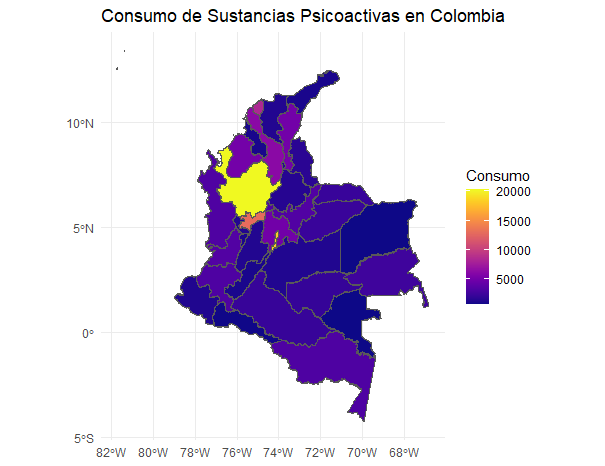
\includegraphics{images/Mapa de calor.png}

El cual resulta de codigo y herramientas, como se ve a continuación:

Mostrar/Ocultar Código

\begin{Shaded}
\begin{Highlighting}[]
\FunctionTok{library}\NormalTok{(sf)}
\FunctionTok{library}\NormalTok{(ggplot2)}
\FunctionTok{library}\NormalTok{(readr)}
\FunctionTok{library}\NormalTok{(dplyr)}
\FunctionTok{library}\NormalTok{(viridis)}

\NormalTok{orden\_departamentos }\OtherTok{\textless{}{-}} \FunctionTok{data.frame}\NormalTok{(}
  \AttributeTok{departamentos =} \FunctionTok{c}\NormalTok{(}\StringTok{"VAUPÉS"}\NormalTok{, }\StringTok{"ANTIOQUIA"}\NormalTok{, }\StringTok{"ATLÁNTICO"}\NormalTok{, }\StringTok{"BOGOTÁ, D.C."}\NormalTok{, }\StringTok{"BOLÍVAR"}\NormalTok{, }\StringTok{"BOYACÁ"}\NormalTok{, }\StringTok{"CALDAS"}\NormalTok{, }\StringTok{"CAQUETÁ"}\NormalTok{, }\StringTok{"CAUCA"}\NormalTok{, }\StringTok{"CESAR"}\NormalTok{, }\StringTok{"CÓRDOBA"}\NormalTok{, }\StringTok{"CUNDINAMARCA"}\NormalTok{, }\StringTok{"CHOCÓ"}\NormalTok{, }\StringTok{"HUILA"}\NormalTok{, }\StringTok{"LA GUAJIRA"}\NormalTok{, }\StringTok{"MAGDALENA"}\NormalTok{, }\StringTok{"META"}\NormalTok{, }\StringTok{"NARIÑO"}\NormalTok{, }\StringTok{"NORTE DE SANTANDER"}\NormalTok{, }\StringTok{"QUINDIO"}\NormalTok{, }\StringTok{"RISARALDA"}\NormalTok{, }\StringTok{"SANTANDER"}\NormalTok{, }\StringTok{"SUCRE"}\NormalTok{, }\StringTok{"TOLIMA"}\NormalTok{, }\StringTok{"VALLE DEL CAUCA"}\NormalTok{, }\StringTok{"ARAUCA"}\NormalTok{, }\StringTok{"CASANARE"}\NormalTok{, }\StringTok{"PUTUMAYO"}\NormalTok{, }\StringTok{"GUAINÍA"}\NormalTok{, }\StringTok{"GUAVIARE"}\NormalTok{, }\StringTok{"VICHADA"}\NormalTok{, }\StringTok{"AMAZONAS"}\NormalTok{),}
  \AttributeTok{consumo\_total =} \FunctionTok{c}\NormalTok{(total\_vaupes, total\_antioquia, total\_atlantico, total\_bogota, total\_bolivar,total\_boyaca, total\_caldas, total\_caqueta, total\_cauca, total\_cesar, total\_cordoba, total\_cundinamarca, total\_choco, total\_huila, total\_guajira, total\_magdalena, total\_meta, total\_nariño, total\_nsantander, total\_quindio, total\_risaralda, total\_santander, total\_sucre, total\_tolima, total\_vcauca, total\_arauca, total\_casanare, total\_putumayo, total\_guania, total\_guaviare, total\_vichada, total\_amazonas))}

\NormalTok{mapa\_consumo }\OtherTok{\textless{}{-}}\NormalTok{ mapa\_colombia\_codigo }\SpecialCharTok{\%\textgreater{}\%}
  \FunctionTok{left\_join}\NormalTok{(orden\_departamentos, }\AttributeTok{by =} \FunctionTok{c}\NormalTok{(}\StringTok{"DPTO\_CNMBR"} \OtherTok{=} \StringTok{"departamentos"}\NormalTok{)) }

\FunctionTok{ggplot}\NormalTok{(}\AttributeTok{data =}\NormalTok{ mapa\_consumo) }\SpecialCharTok{+}
  \FunctionTok{geom\_sf}\NormalTok{(}\FunctionTok{aes}\NormalTok{(}\AttributeTok{fill =}\NormalTok{ consumo\_total)) }\SpecialCharTok{+}
  \FunctionTok{scale\_fill\_viridis}\NormalTok{(}\AttributeTok{option =} \StringTok{"plasma"}\NormalTok{, }\AttributeTok{na.value =} \StringTok{"grey"}\NormalTok{) }\SpecialCharTok{+}
  \FunctionTok{theme\_minimal}\NormalTok{() }\SpecialCharTok{+}
  \FunctionTok{labs}\NormalTok{(}\AttributeTok{title =} \StringTok{"Consumo de Sustancias Psicoactivas en Colombia"}\NormalTok{,}
       \AttributeTok{fill =} \StringTok{"Consumo"}\NormalTok{)}
\end{Highlighting}
\end{Shaded}

3.3.~ Se eligen los 4 departamentos donde se observan los valores de
mayor consumo en total de sustancias psicoactivas, los cuales son
Antioquia, Santander y Valle del Cauca, adicional a ello la ciudad de
Bogotá D.C, en donde se realiza el análisis de cada una de las variables
nombradas anteriormente por cada una de las sustancias psicoactivas,
cuyos resultados darán pie a la discusión y respuesta de la pregunta de
investigación.

\section{Analisis de consumo basado en
Santander}\label{analisis-de-consumo-basado-en-santander}

Luego de realizar todo el proceso anterior con los datos de Santander,
filtrando los datos según la ocupación, el estado de salud, si pertenece
a alguna minoría, el nivel educativo máximo alcanzado, su orientación
sexual, identidad de género, el sexo de nacimiento y la edad, separando
cada una por la sustancia que consume la persona, antes se realizaron
\emph{mapas de calor} del consumo de por cada sustancia en el
departamento analizando cada uno de sus municipios:

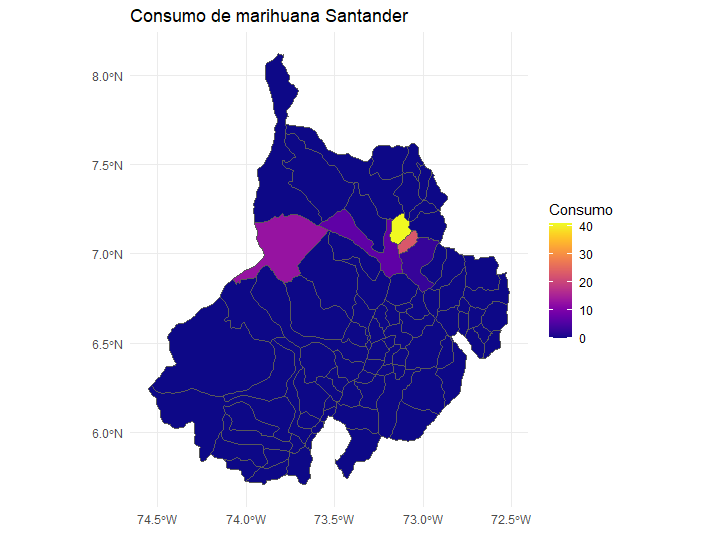
\includegraphics{images/Mapa de consumo de marihuana en santander.png}

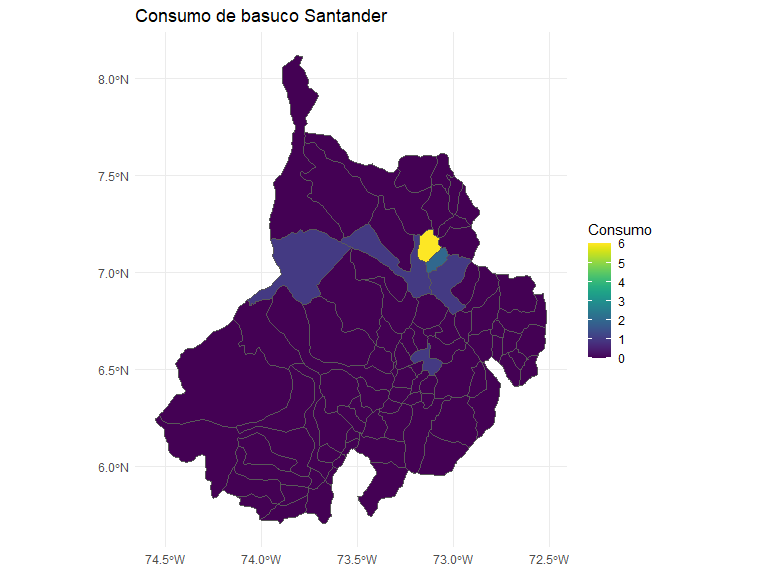
\includegraphics{images/Mapa consumo de basuco en santander.png}

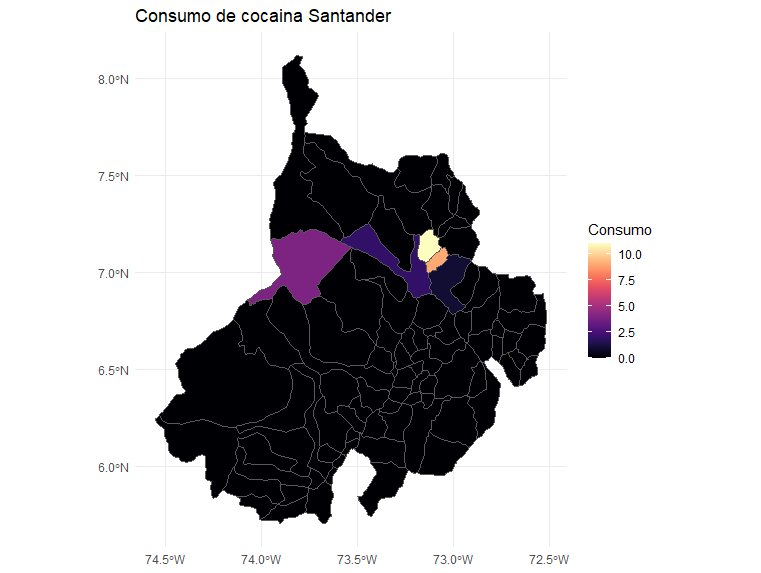
\includegraphics{images/Mapa consumo de cocaina en santander.png}

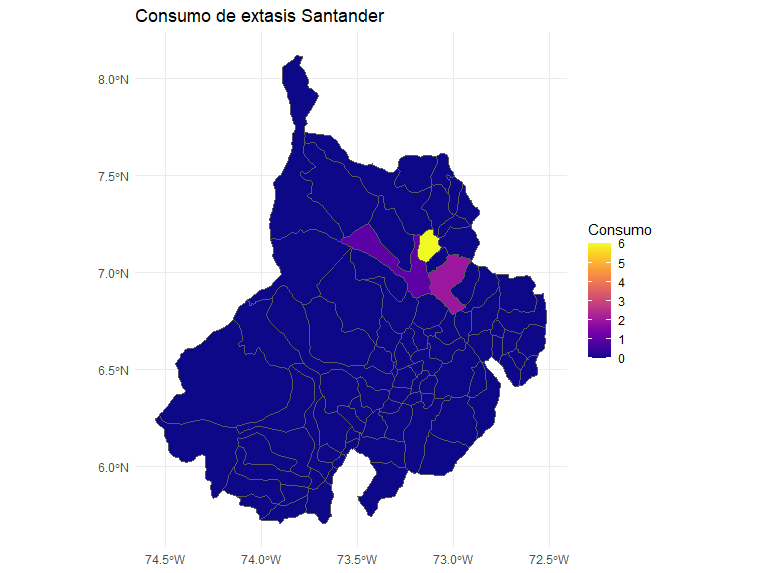
\includegraphics{images/Mapa consumo de extasis en satander.png}

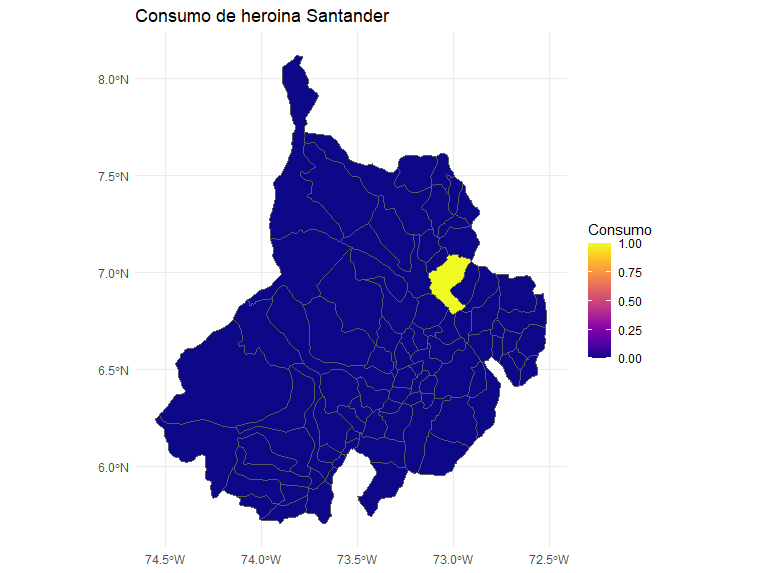
\includegraphics{images/Mapa consumo de heroina en santander.png}

para dichos mapa se hizo uso de librerias y código mostrado a
continuación (donde se encuentren ``\ldots{}'' correponde a datos
adicionales que no se muestran pero que son necesarios):

Mostrar/Ocultar Código

\begin{Shaded}
\begin{Highlighting}[]
\FunctionTok{library}\NormalTok{(readr)}
\FunctionTok{library}\NormalTok{(dplyr)}
\FunctionTok{library}\NormalTok{(sf)}
\FunctionTok{library}\NormalTok{(ggplot2)}
\FunctionTok{library}\NormalTok{(viridis)}

\NormalTok{municipios\_santander }\OtherTok{\textless{}{-}} \FunctionTok{c}\NormalTok{(}
  \StringTok{"Aguada"} \OtherTok{=} \StringTok{"68013"}\NormalTok{,}
  \StringTok{"Albania"} \OtherTok{=} \StringTok{"68020"}\NormalTok{,}
  \StringTok{"Aratoca"} \OtherTok{=} \StringTok{"68051"}\NormalTok{,}
  \StringTok{"Barbosa"} \OtherTok{=} \StringTok{"68077"}\NormalTok{,}
  \StringTok{"Barichara"} \OtherTok{=} \StringTok{"68079"}\NormalTok{,}\StringTok{"..."}\NormalTok{)}

\NormalTok{datos\_consumidores }\OtherTok{\textless{}{-}} \FunctionTok{list}\NormalTok{()}

\ControlFlowTok{for}\NormalTok{ (municipio }\ControlFlowTok{in} \FunctionTok{names}\NormalTok{(municipios\_santander)) \{}
\NormalTok{  codigo }\OtherTok{\textless{}{-}}\NormalTok{ municipios\_santander[municipio]}
  
\NormalTok{  datos\_consumidores[[municipio]] }\OtherTok{\textless{}{-}}\NormalTok{ csv\_con\_valores\_completos}\SpecialCharTok{$}\NormalTok{consumidores\_extasis\_santander.csv }\SpecialCharTok{\%\textgreater{}\%}
    \FunctionTok{filter}\NormalTok{(}\FunctionTok{startsWith}\NormalTok{(}\FunctionTok{as.character}\NormalTok{(csv\_con\_valores\_completos}\SpecialCharTok{$}\NormalTok{consumidores\_extasis\_santander.csv}\SpecialCharTok{$}\NormalTok{Depmuni), codigo))}
\NormalTok{\}}

\NormalTok{total\_bucaramanga }\OtherTok{\textless{}{-}} \FunctionTok{nrow}\NormalTok{(datos\_consumidores[[}\StringTok{"Bucaramanga"}\NormalTok{]])}
\NormalTok{total\_aguada }\OtherTok{\textless{}{-}} \FunctionTok{nrow}\NormalTok{(datos\_consumidores[[}\StringTok{"Aguada"}\NormalTok{]])}
\NormalTok{total\_albania }\OtherTok{\textless{}{-}} \FunctionTok{nrow}\NormalTok{(datos\_consumidores[[}\StringTok{"Albania"}\NormalTok{]])}
\NormalTok{total\_aratoca }\OtherTok{\textless{}{-}} \FunctionTok{nrow}\NormalTok{(datos\_consumidores[[}\StringTok{"Aratoca"}\NormalTok{]])}
\StringTok{"....."}

\NormalTok{consumo\_extasis\_por\_municipio\_santander }\OtherTok{\textless{}{-}} \FunctionTok{data.frame}\NormalTok{(}
  \AttributeTok{municipios =} \FunctionTok{c}\NormalTok{(}\StringTok{"ZAPATOCA"}\NormalTok{, }\StringTok{"PUERTO WILCHES"}\NormalTok{, }\StringTok{"MALAGA"}\NormalTok{, }\StringTok{"CARCASI"}\NormalTok{, }\StringTok{"LA BELLEZA"}\NormalTok{, }\StringTok{"CAPITANEJO"}\NormalTok{, }\StringTok{"SANTA HELENA DEL OPON"}\NormalTok{, }\StringTok{"LA PAZ"}\NormalTok{, }\StringTok{"SUAITA"}\NormalTok{, }\StringTok{"MATANZA"}\NormalTok{, }
                 \StringTok{"LOS SANTOS"}\NormalTok{, }\StringTok{"GALAN"}\NormalTok{, }\StringTok{"SUCRE"}\NormalTok{, }\StringTok{"PUENTE NACIONAL"}\NormalTok{, }\StringTok{"GAMBITA"}\NormalTok{, }\StringTok{"MAGDALENA"}\NormalTok{, }\StringTok{"GUAVATA"}\NormalTok{, }\StringTok{"MOLAGAVITA"}\NormalTok{, }\StringTok{"BARBOSA"}\NormalTok{, }\StringTok{"..."}\NormalTok{),}
  \AttributeTok{consumo\_total =} \FunctionTok{c}\NormalTok{(}\DecValTok{0}\NormalTok{,}\DecValTok{0}\NormalTok{,}\DecValTok{0}\NormalTok{,}\DecValTok{0}\NormalTok{,}\DecValTok{0}\NormalTok{,}\DecValTok{0}\NormalTok{,}\DecValTok{0}\NormalTok{,}\DecValTok{0}\NormalTok{,}\DecValTok{0}\NormalTok{,}\DecValTok{0}\NormalTok{,}\StringTok{"..."}\NormalTok{))}

\NormalTok{mapa\_santander }\OtherTok{\textless{}{-}} \FunctionTok{st\_read}\NormalTok{(}\StringTok{"C:/Users/ASUS/Desktop/Estadistica/Estadistica\_1\_\_Grupo\_E2\_\_\_PROYECTO\_\_INVESTIGACION\_\_\_DAVID\_ALEJANDRO\_ZAPATA\_TORO/DATOS DANE/Datos separados/Mapeo/Mapas/shapes/shapes.shp"}\NormalTok{)}

\NormalTok{mapa\_santander\_nombre\_municipio }\OtherTok{\textless{}{-}}\NormalTok{ mapa\_santander[,}\DecValTok{6}\NormalTok{]}

\NormalTok{mapa\_consumo\_extasis\_santander }\OtherTok{\textless{}{-}}\NormalTok{ mapa\_santander\_nombre\_municipio }\SpecialCharTok{\%\textgreater{}\%}
  \FunctionTok{left\_join}\NormalTok{(consumo\_extasis\_por\_municipio\_santander, }\AttributeTok{by =} \FunctionTok{c}\NormalTok{(}\StringTok{"nombre\_mpi"} \OtherTok{=} \StringTok{"municipios"}\NormalTok{)) }

\FunctionTok{ggplot}\NormalTok{(}\AttributeTok{data =}\NormalTok{ mapa\_consumo\_extasis\_santander) }\SpecialCharTok{+}
  \FunctionTok{geom\_sf}\NormalTok{(}\FunctionTok{aes}\NormalTok{(}\AttributeTok{fill =}\NormalTok{ consumo\_total)) }\SpecialCharTok{+}
  \FunctionTok{scale\_fill\_viridis}\NormalTok{(}\AttributeTok{option =} \StringTok{"plasma"}\NormalTok{, }\AttributeTok{na.value =} \StringTok{"grey"}\NormalTok{) }\SpecialCharTok{+}
  \FunctionTok{theme\_minimal}\NormalTok{() }\SpecialCharTok{+}
  \FunctionTok{labs}\NormalTok{(}\AttributeTok{title =} \StringTok{"Consumo de extasis Santander"}\NormalTok{,}
       \AttributeTok{fill =} \StringTok{"Consumo"}\NormalTok{)}
\end{Highlighting}
\end{Shaded}

El formato anterior se uso para cada uno de los mapas generados por
sustancia psicoactiva a estudiar.

De este mapeo podemos observar que la mayoria de consumidores de
sustancias psicoactivas en Santander se encuentran en el area
metropolitana que esta conformada por, Floridablanca, Bucaramanga,
Piedecuesta y Girón.

\section{Analisis de variables}\label{analisis-de-variables}

Para nuestro informe se sacaron graficas basandonos en las siguientes
variables:

\begin{enumerate}
\def\labelenumi{\arabic{enumi}.}
\tightlist
\item
  Consumo de sustancias por primera vez
\end{enumerate}

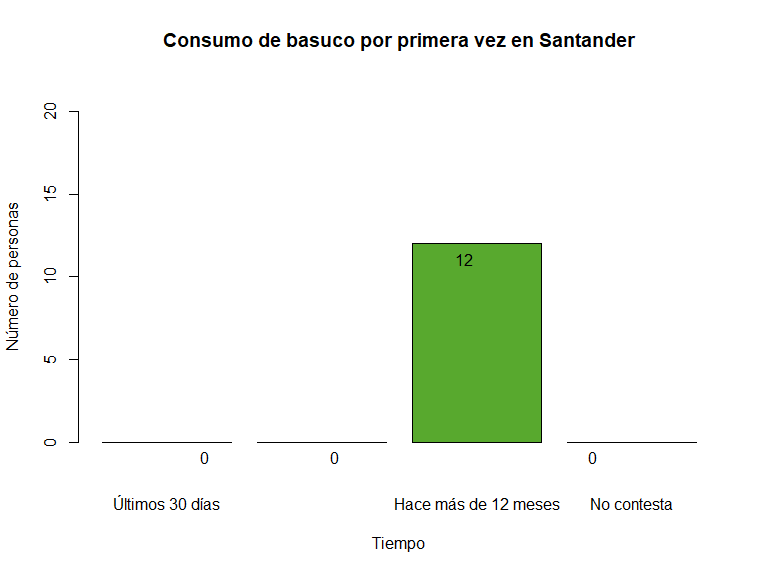
\includegraphics{images/basuco 1 santander.png}

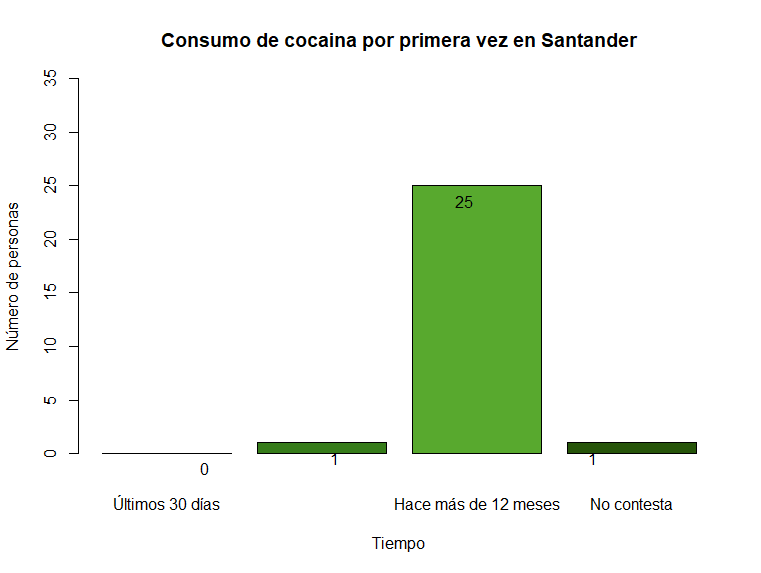
\includegraphics{images/cocaina 1 santander.png}

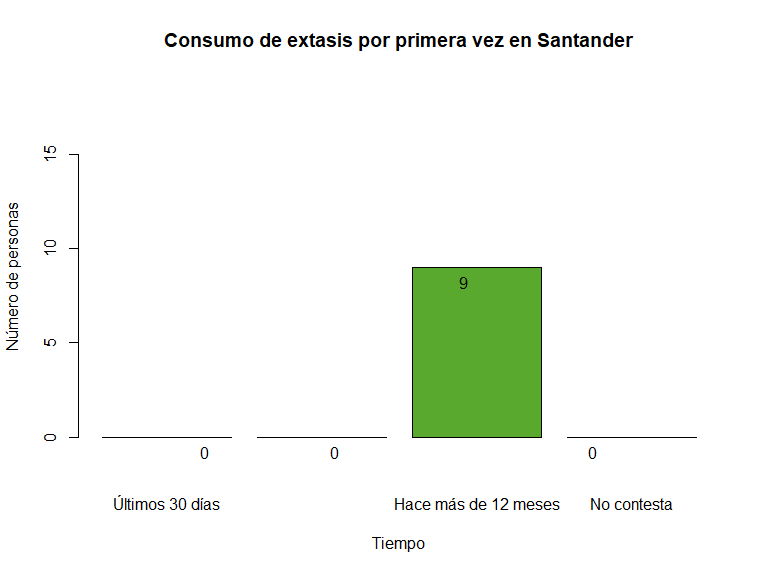
\includegraphics{images/extasis 1 santander.png}

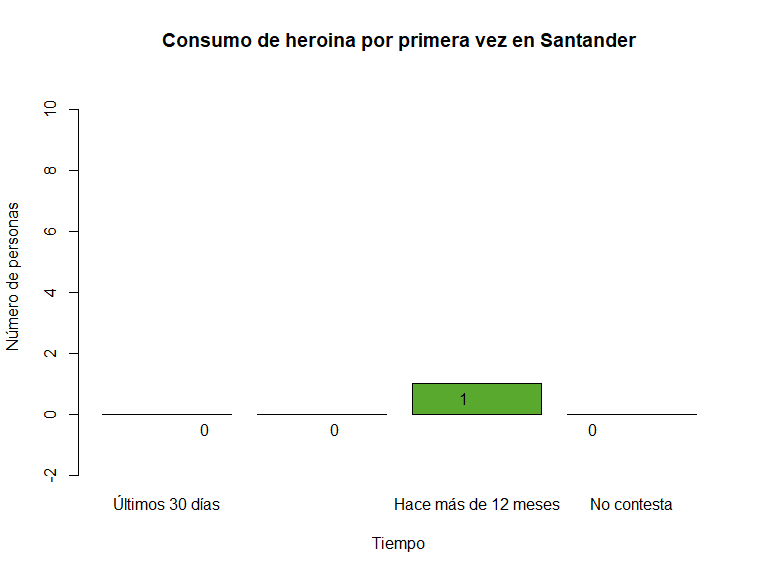
\includegraphics{images/heroina 1 santander.png}

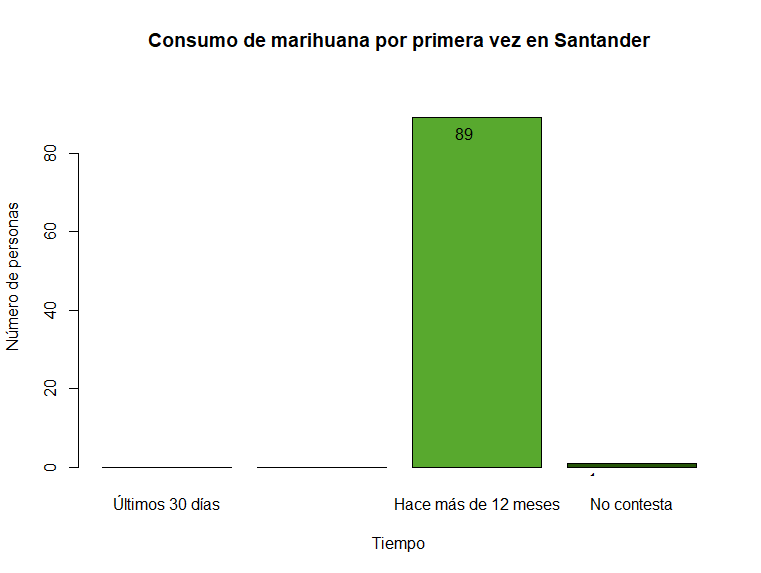
\includegraphics{images/marihuana 1 santander.png}

La rutina para graficación y analisis es la misma para cada sustancia,
variando unicamente en el nombre de la columna donde cada sustancia
variaba de nombre.

Mostrar/Ocultar Código

\begin{Shaded}
\begin{Highlighting}[]
\NormalTok{columna }\OtherTok{\textless{}{-}} \StringTok{"M\_01"}
\NormalTok{valores}\OtherTok{\textless{}{-}}\FunctionTok{c}\NormalTok{(}\StringTok{"1"}\NormalTok{, }\StringTok{"2"}\NormalTok{, }\StringTok{"3"}\NormalTok{, }\StringTok{"9"}\NormalTok{)}
\NormalTok{etiquetas }\OtherTok{\textless{}{-}} \FunctionTok{c}\NormalTok{(}
  \StringTok{"Últimos 30 días"}\NormalTok{,}
  \StringTok{"Hace más de +30 días,{-}12 meses"}\NormalTok{,}
  \StringTok{"Hace más de 12 meses"}\NormalTok{,}
  \StringTok{"No contesta"}
\NormalTok{)}

\NormalTok{cuentas }\OtherTok{\textless{}{-}} \FunctionTok{c}\NormalTok{()}

\ControlFlowTok{for}\NormalTok{ (valor }\ControlFlowTok{in}\NormalTok{ valores) \{}
\NormalTok{  cuenta }\OtherTok{\textless{}{-}} \FunctionTok{sum}\NormalTok{(santander\_basuco[[columna]] }\SpecialCharTok{==}\NormalTok{ valor)}
\NormalTok{  cuentas }\OtherTok{\textless{}{-}} \FunctionTok{c}\NormalTok{(cuentas, cuenta) }
  \ControlFlowTok{if}\NormalTok{ (valor }\SpecialCharTok{==} \StringTok{"1"}\NormalTok{) \{}
    \FunctionTok{cat}\NormalTok{(}\FunctionTok{sprintf}\NormalTok{(}\StringTok{"Personas que consumieron basuco por primera vez en los últimos 30 días en Santander: \%s}\SpecialCharTok{\textbackslash{}n}\StringTok{"}\NormalTok{, cuenta))}
\NormalTok{  \} }\ControlFlowTok{else} \ControlFlowTok{if}\NormalTok{ (valor }\SpecialCharTok{==} \StringTok{"2"}\NormalTok{) \{}
    \FunctionTok{cat}\NormalTok{(}\FunctionTok{sprintf}\NormalTok{(}\StringTok{"Personas que consumieron basuco por primera vez hace más de 30 días pero menos de 12 meses en Santander: \%s}\SpecialCharTok{\textbackslash{}n}\StringTok{"}\NormalTok{, cuenta))}
\NormalTok{  \} }\ControlFlowTok{else} \ControlFlowTok{if}\NormalTok{ (valor }\SpecialCharTok{==} \StringTok{"3"}\NormalTok{) \{}
    \FunctionTok{cat}\NormalTok{(}\FunctionTok{sprintf}\NormalTok{(}\StringTok{"Personas que consumieron basuco por primera vez hace más de 12 meses en Santander: \%s}\SpecialCharTok{\textbackslash{}n}\StringTok{"}\NormalTok{, cuenta))}
\NormalTok{  \} }\ControlFlowTok{else} \ControlFlowTok{if}\NormalTok{ (valor }\SpecialCharTok{==} \StringTok{"9"}\NormalTok{) \{}
    \FunctionTok{cat}\NormalTok{(}\FunctionTok{sprintf}\NormalTok{(}\StringTok{"Personas que no contesta cuando consumieron basuco por primera vez en Santander: \%s}\SpecialCharTok{\textbackslash{}n}\StringTok{"}\NormalTok{, cuenta))}
\NormalTok{  \}}
\NormalTok{\}}

\FunctionTok{barplot}\NormalTok{(}
\NormalTok{  cuentas,}
  \AttributeTok{names.arg =}\NormalTok{ etiquetas,}
  \AttributeTok{col =} \FunctionTok{c}\NormalTok{(}\StringTok{"\#c9ecaf"}\NormalTok{, }\StringTok{"\#367c1a"}\NormalTok{, }\StringTok{"\#58a92e"}\NormalTok{, }\StringTok{"\#265409"}\NormalTok{),}
  \AttributeTok{main =} \StringTok{"Consumo de basuco por primera vez en Santander"}\NormalTok{,}
  \AttributeTok{xlab =} \StringTok{"Tiempo"}\NormalTok{,}
  \AttributeTok{ylab =} \StringTok{"Número de personas"}\NormalTok{,}
  \AttributeTok{ylim =} \FunctionTok{c}\NormalTok{(}\SpecialCharTok{{-}}\DecValTok{2}\NormalTok{, }\FunctionTok{max}\NormalTok{(cuentas) }\SpecialCharTok{+} \DecValTok{10}\NormalTok{)}
\NormalTok{)}
\end{Highlighting}
\end{Shaded}

\begin{enumerate}
\def\labelenumi{\arabic{enumi}.}
\setcounter{enumi}{1}
\tightlist
\item
  Consumo y trabajo:
\end{enumerate}

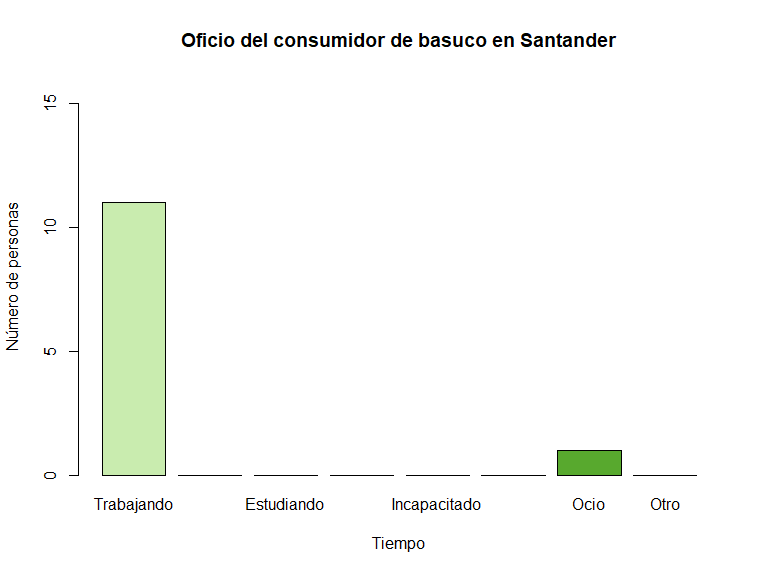
\includegraphics{images/Basuco oficio Santander.png}

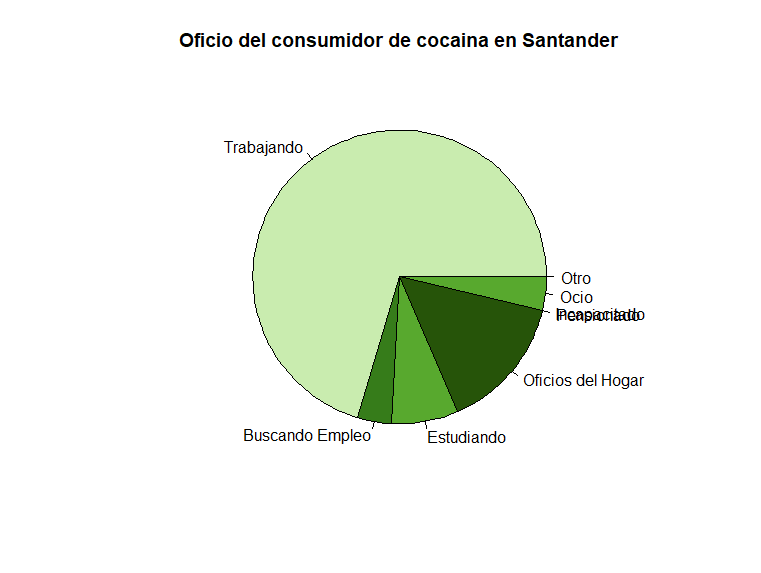
\includegraphics{images/cocaina oficio santander.png}

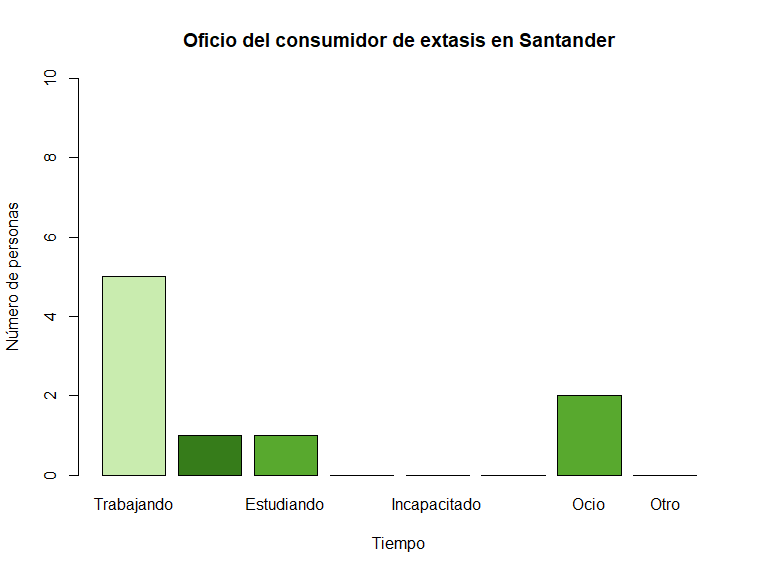
\includegraphics{images/extasis oficio santander.png}

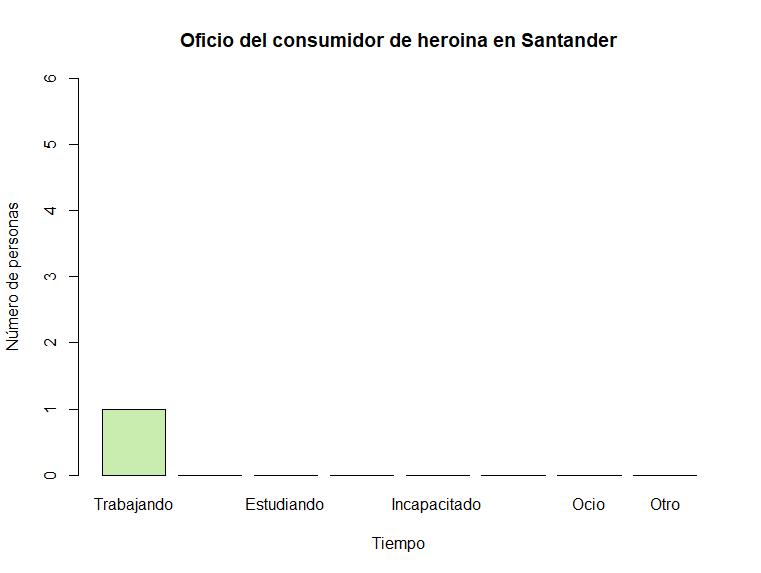
\includegraphics{images/heroina oficio santander.png}

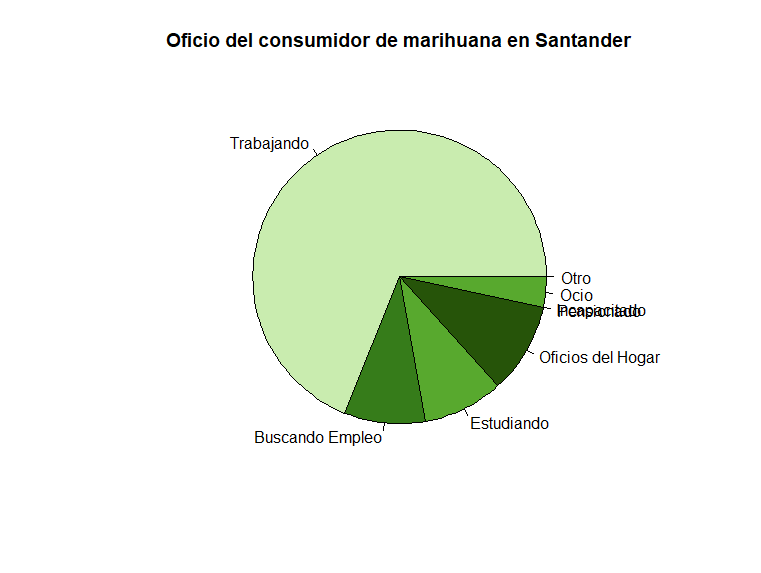
\includegraphics{images/marihuana oficio santander.png}

Mostrar/Ocultar Código

\begin{Shaded}
\begin{Highlighting}[]
\NormalTok{columna }\OtherTok{\textless{}{-}} \StringTok{"D\_02"}
\NormalTok{valores}\OtherTok{\textless{}{-}}\FunctionTok{c}\NormalTok{(}\StringTok{"1"}\NormalTok{, }\StringTok{"2"}\NormalTok{, }\StringTok{"3"}\NormalTok{, }\StringTok{"4"}\NormalTok{,}\StringTok{"5"}\NormalTok{,}\StringTok{"6"}\NormalTok{,}\StringTok{"7"}\NormalTok{,}\StringTok{"8"}\NormalTok{)}
\NormalTok{etiquetas }\OtherTok{\textless{}{-}} \FunctionTok{c}\NormalTok{(}
  \StringTok{"Trabajando"}\NormalTok{,}
  \StringTok{"Buscando Empleo"}\NormalTok{,}
  \StringTok{"Estudiando"}\NormalTok{,}
  \StringTok{"Oficios del Hogar"}\NormalTok{,}
  \StringTok{"Incapacitado"}\NormalTok{,}
  \StringTok{"Pensionado"}\NormalTok{,}
  \StringTok{"Ocio"}\NormalTok{,}
  \StringTok{"Otro"}
\NormalTok{)}

\NormalTok{cuentas }\OtherTok{\textless{}{-}} \FunctionTok{c}\NormalTok{()}

\ControlFlowTok{for}\NormalTok{ (valor }\ControlFlowTok{in}\NormalTok{ valores) \{}
\NormalTok{  cuenta }\OtherTok{\textless{}{-}} \FunctionTok{sum}\NormalTok{(santander\_basuco[[columna]] }\SpecialCharTok{==}\NormalTok{ valor)}
\NormalTok{  cuentas }\OtherTok{\textless{}{-}} \FunctionTok{c}\NormalTok{(cuentas, cuenta)  }\CommentTok{\# Agregar cada cuenta al vector}
  
  \ControlFlowTok{if}\NormalTok{ (valor }\SpecialCharTok{==} \StringTok{"1"}\NormalTok{) \{}
    \FunctionTok{cat}\NormalTok{(}\FunctionTok{sprintf}\NormalTok{(}\StringTok{"Personas que trabajan y consumen basuco: \%s}\SpecialCharTok{\textbackslash{}n}\StringTok{"}\NormalTok{, cuenta))}
\NormalTok{  \} }\ControlFlowTok{else} \ControlFlowTok{if}\NormalTok{ (valor }\SpecialCharTok{==} \StringTok{"2"}\NormalTok{) \{}
    \FunctionTok{cat}\NormalTok{(}\FunctionTok{sprintf}\NormalTok{(}\StringTok{"Personas que buscan empleo y consumen basuco: \%s}\SpecialCharTok{\textbackslash{}n}\StringTok{"}\NormalTok{, cuenta))}
\NormalTok{  \} }\ControlFlowTok{else} \ControlFlowTok{if}\NormalTok{ (valor }\SpecialCharTok{==} \StringTok{"3"}\NormalTok{) \{}
    \FunctionTok{cat}\NormalTok{(}\FunctionTok{sprintf}\NormalTok{(}\StringTok{"Personas que estudian y consumen basuco: \%s}\SpecialCharTok{\textbackslash{}n}\StringTok{"}\NormalTok{, cuenta))}
\NormalTok{  \} }\ControlFlowTok{else} \ControlFlowTok{if}\NormalTok{ (valor }\SpecialCharTok{==} \StringTok{"4"}\NormalTok{) \{}
    \FunctionTok{cat}\NormalTok{(}\FunctionTok{sprintf}\NormalTok{(}\StringTok{"Personas que se encargan del oficio del hogar y consumen basuco: \%s}\SpecialCharTok{\textbackslash{}n}\StringTok{"}\NormalTok{, cuenta))}
\NormalTok{  \} }\ControlFlowTok{else} \ControlFlowTok{if}\NormalTok{ (valor }\SpecialCharTok{==} \StringTok{"5"}\NormalTok{) \{}
    \FunctionTok{cat}\NormalTok{(}\FunctionTok{sprintf}\NormalTok{(}\StringTok{"Personas que estan incapacitados y consumen basuco: \%s}\SpecialCharTok{\textbackslash{}n}\StringTok{"}\NormalTok{, cuenta))}
\NormalTok{  \} }\ControlFlowTok{else} \ControlFlowTok{if}\NormalTok{ (valor }\SpecialCharTok{==} \StringTok{"6"}\NormalTok{) \{}
    \FunctionTok{cat}\NormalTok{(}\FunctionTok{sprintf}\NormalTok{(}\StringTok{"Personas que estan pensionados y consumen basuco: \%s}\SpecialCharTok{\textbackslash{}n}\StringTok{"}\NormalTok{, cuenta))}
\NormalTok{  \} }\ControlFlowTok{else} \ControlFlowTok{if}\NormalTok{ (valor }\SpecialCharTok{==} \StringTok{"7"}\NormalTok{) \{}
    \FunctionTok{cat}\NormalTok{(}\FunctionTok{sprintf}\NormalTok{(}\StringTok{"Personas que se dedican al ocio y consumen basuco: \%s}\SpecialCharTok{\textbackslash{}n}\StringTok{"}\NormalTok{, cuenta))}
\NormalTok{  \} }\ControlFlowTok{else} \ControlFlowTok{if}\NormalTok{ (valor }\SpecialCharTok{==} \StringTok{"8"}\NormalTok{) \{}
    \FunctionTok{cat}\NormalTok{(}\FunctionTok{sprintf}\NormalTok{(}\StringTok{"Personas que se dedican a otras actividades y consumen basuco: \%s}\SpecialCharTok{\textbackslash{}n}\StringTok{"}\NormalTok{, cuenta))}
\NormalTok{  \}}
  
\NormalTok{\}}

\FunctionTok{barplot}\NormalTok{(}
\NormalTok{  cuentas,}
  \AttributeTok{names.arg =}\NormalTok{ etiquetas,}
  \AttributeTok{col =} \FunctionTok{c}\NormalTok{(}\StringTok{"\#c9ecaf"}\NormalTok{, }\StringTok{"\#367c1a"}\NormalTok{, }\StringTok{"\#58a92e"}\NormalTok{, }\StringTok{"\#265409"}\NormalTok{,}\StringTok{"\#c9ecaf"}\NormalTok{, }\StringTok{"\#367c1a"}\NormalTok{, }\StringTok{"\#58a92e"}\NormalTok{, }\StringTok{"\#265409"}\NormalTok{),}
  \AttributeTok{main =} \StringTok{"Oficio del consumidor de basuco en Santander"}\NormalTok{,}
  \AttributeTok{xlab =} \StringTok{"Tiempo"}\NormalTok{,}
  \AttributeTok{ylab =} \StringTok{"Número de personas"}\NormalTok{,}
  \AttributeTok{ylim =} \FunctionTok{c}\NormalTok{(}\DecValTok{0}\NormalTok{, }\FunctionTok{max}\NormalTok{(cuentas) }\SpecialCharTok{+} \DecValTok{5}\NormalTok{)}
\NormalTok{)}

\CommentTok{\#Oficio del consumidor cocaina }
\NormalTok{cuentas }\OtherTok{\textless{}{-}} \FunctionTok{c}\NormalTok{()}
\ControlFlowTok{for}\NormalTok{ (valor }\ControlFlowTok{in}\NormalTok{ valores) \{}
\NormalTok{  cuenta }\OtherTok{\textless{}{-}} \FunctionTok{sum}\NormalTok{(santander\_cocaina[[columna]] }\SpecialCharTok{==}\NormalTok{ valor)}
\NormalTok{  cuentas }\OtherTok{\textless{}{-}} \FunctionTok{c}\NormalTok{(cuentas, cuenta)  }\CommentTok{\# Agregar cada cuenta al vector}
  
  \ControlFlowTok{if}\NormalTok{ (valor }\SpecialCharTok{==} \StringTok{"1"}\NormalTok{) \{}
    \FunctionTok{cat}\NormalTok{(}\FunctionTok{sprintf}\NormalTok{(}\StringTok{"Personas que trabajan y consumen cocaina: \%s}\SpecialCharTok{\textbackslash{}n}\StringTok{"}\NormalTok{, cuenta))}
\NormalTok{  \} }\ControlFlowTok{else} \ControlFlowTok{if}\NormalTok{ (valor }\SpecialCharTok{==} \StringTok{"2"}\NormalTok{) \{}
    \FunctionTok{cat}\NormalTok{(}\FunctionTok{sprintf}\NormalTok{(}\StringTok{"Personas que buscan empleo y consumen cocaina: \%s}\SpecialCharTok{\textbackslash{}n}\StringTok{"}\NormalTok{, cuenta))}
\NormalTok{  \} }\ControlFlowTok{else} \ControlFlowTok{if}\NormalTok{ (valor }\SpecialCharTok{==} \StringTok{"3"}\NormalTok{) \{}
    \FunctionTok{cat}\NormalTok{(}\FunctionTok{sprintf}\NormalTok{(}\StringTok{"Personas que estudian y consumen cocaina: \%s}\SpecialCharTok{\textbackslash{}n}\StringTok{"}\NormalTok{, cuenta))}
\NormalTok{  \} }\ControlFlowTok{else} \ControlFlowTok{if}\NormalTok{ (valor }\SpecialCharTok{==} \StringTok{"4"}\NormalTok{) \{}
    \FunctionTok{cat}\NormalTok{(}\FunctionTok{sprintf}\NormalTok{(}\StringTok{"Personas que se encargan del oficio del hogar y consumen cocaina: \%s}\SpecialCharTok{\textbackslash{}n}\StringTok{"}\NormalTok{, cuenta))}
\NormalTok{  \} }\ControlFlowTok{else} \ControlFlowTok{if}\NormalTok{ (valor }\SpecialCharTok{==} \StringTok{"5"}\NormalTok{) \{}
    \FunctionTok{cat}\NormalTok{(}\FunctionTok{sprintf}\NormalTok{(}\StringTok{"Personas que estan incapacitados y consumen cocaina: \%s}\SpecialCharTok{\textbackslash{}n}\StringTok{"}\NormalTok{, cuenta))}
\NormalTok{  \} }\ControlFlowTok{else} \ControlFlowTok{if}\NormalTok{ (valor }\SpecialCharTok{==} \StringTok{"6"}\NormalTok{) \{}
    \FunctionTok{cat}\NormalTok{(}\FunctionTok{sprintf}\NormalTok{(}\StringTok{"Personas que estan pensionados y consumen cocaina: \%s}\SpecialCharTok{\textbackslash{}n}\StringTok{"}\NormalTok{, cuenta))}
\NormalTok{  \} }\ControlFlowTok{else} \ControlFlowTok{if}\NormalTok{ (valor }\SpecialCharTok{==} \StringTok{"7"}\NormalTok{) \{}
    \FunctionTok{cat}\NormalTok{(}\FunctionTok{sprintf}\NormalTok{(}\StringTok{"Personas que se dedican al ocio y consumen cocaina: \%s}\SpecialCharTok{\textbackslash{}n}\StringTok{"}\NormalTok{, cuenta))}
\NormalTok{  \} }\ControlFlowTok{else} \ControlFlowTok{if}\NormalTok{ (valor }\SpecialCharTok{==} \StringTok{"8"}\NormalTok{) \{}
    \FunctionTok{cat}\NormalTok{(}\FunctionTok{sprintf}\NormalTok{(}\StringTok{"Personas que se dedican a otras actividades y consumen cocaina: \%s}\SpecialCharTok{\textbackslash{}n}\StringTok{"}\NormalTok{, cuenta))}
\NormalTok{  \}}
  
\NormalTok{\}}

\FunctionTok{pie}\NormalTok{(}
\NormalTok{  cuentas,}
  \AttributeTok{labels =}\NormalTok{ etiquetas,}
  \AttributeTok{main =} \StringTok{"Oficio del consumidor de cocaina en Santander"}\NormalTok{,}
  \AttributeTok{col =} \FunctionTok{c}\NormalTok{(}\StringTok{"\#c9ecaf"}\NormalTok{, }\StringTok{"\#367c1a"}\NormalTok{, }\StringTok{"\#58a92e"}\NormalTok{, }\StringTok{"\#265409"}\NormalTok{,}\StringTok{"\#c9ecaf"}\NormalTok{, }\StringTok{"\#367c1a"}\NormalTok{, }\StringTok{"\#58a92e"}\NormalTok{, }\StringTok{"\#265409"}\NormalTok{)}
\NormalTok{)}


\CommentTok{\#Oficio del consumidor extasis }
\NormalTok{cuentas }\OtherTok{\textless{}{-}} \FunctionTok{c}\NormalTok{()}
\ControlFlowTok{for}\NormalTok{ (valor }\ControlFlowTok{in}\NormalTok{ valores) \{}
\NormalTok{  cuenta }\OtherTok{\textless{}{-}} \FunctionTok{sum}\NormalTok{(santander\_extasis[[columna]] }\SpecialCharTok{==}\NormalTok{ valor)}
\NormalTok{  cuentas }\OtherTok{\textless{}{-}} \FunctionTok{c}\NormalTok{(cuentas, cuenta)  }\CommentTok{\# Agregar cada cuenta al vector}
  \ControlFlowTok{if}\NormalTok{ (valor }\SpecialCharTok{==} \StringTok{"1"}\NormalTok{) \{}
    \FunctionTok{cat}\NormalTok{(}\FunctionTok{sprintf}\NormalTok{(}\StringTok{"Personas que trabajan y consumen extasis: \%s}\SpecialCharTok{\textbackslash{}n}\StringTok{"}\NormalTok{, cuenta))}
\NormalTok{  \} }\ControlFlowTok{else} \ControlFlowTok{if}\NormalTok{ (valor }\SpecialCharTok{==} \StringTok{"2"}\NormalTok{) \{}
    \FunctionTok{cat}\NormalTok{(}\FunctionTok{sprintf}\NormalTok{(}\StringTok{"Personas que buscan empleo y consumen extasis: \%s}\SpecialCharTok{\textbackslash{}n}\StringTok{"}\NormalTok{, cuenta))}
\NormalTok{  \} }\ControlFlowTok{else} \ControlFlowTok{if}\NormalTok{ (valor }\SpecialCharTok{==} \StringTok{"3"}\NormalTok{) \{}
    \FunctionTok{cat}\NormalTok{(}\FunctionTok{sprintf}\NormalTok{(}\StringTok{"Personas que estudian y consumen extasis: \%s}\SpecialCharTok{\textbackslash{}n}\StringTok{"}\NormalTok{, cuenta))}
\NormalTok{  \} }\ControlFlowTok{else} \ControlFlowTok{if}\NormalTok{ (valor }\SpecialCharTok{==} \StringTok{"4"}\NormalTok{) \{}
    \FunctionTok{cat}\NormalTok{(}\FunctionTok{sprintf}\NormalTok{(}\StringTok{"Personas que se encargan del oficio del hogar y consumen extasis: \%s}\SpecialCharTok{\textbackslash{}n}\StringTok{"}\NormalTok{, cuenta))}
\NormalTok{  \} }\ControlFlowTok{else} \ControlFlowTok{if}\NormalTok{ (valor }\SpecialCharTok{==} \StringTok{"5"}\NormalTok{) \{}
    \FunctionTok{cat}\NormalTok{(}\FunctionTok{sprintf}\NormalTok{(}\StringTok{"Personas que estan incapacitados y consumen extasis: \%s}\SpecialCharTok{\textbackslash{}n}\StringTok{"}\NormalTok{, cuenta))}
\NormalTok{  \} }\ControlFlowTok{else} \ControlFlowTok{if}\NormalTok{ (valor }\SpecialCharTok{==} \StringTok{"6"}\NormalTok{) \{}
    \FunctionTok{cat}\NormalTok{(}\FunctionTok{sprintf}\NormalTok{(}\StringTok{"Personas que estan pensionados y consumen extasis: \%s}\SpecialCharTok{\textbackslash{}n}\StringTok{"}\NormalTok{, cuenta))}
\NormalTok{  \} }\ControlFlowTok{else} \ControlFlowTok{if}\NormalTok{ (valor }\SpecialCharTok{==} \StringTok{"7"}\NormalTok{) \{}
    \FunctionTok{cat}\NormalTok{(}\FunctionTok{sprintf}\NormalTok{(}\StringTok{"Personas que se dedican al ocio y consumen extasis: \%s}\SpecialCharTok{\textbackslash{}n}\StringTok{"}\NormalTok{, cuenta))}
\NormalTok{  \} }\ControlFlowTok{else} \ControlFlowTok{if}\NormalTok{ (valor }\SpecialCharTok{==} \StringTok{"8"}\NormalTok{) \{}
    \FunctionTok{cat}\NormalTok{(}\FunctionTok{sprintf}\NormalTok{(}\StringTok{"Personas que se dedican a otras actividades y consumen extasis: \%s}\SpecialCharTok{\textbackslash{}n}\StringTok{"}\NormalTok{, cuenta))}
\NormalTok{  \}}
  
\NormalTok{\}}

\FunctionTok{barplot}\NormalTok{(}
\NormalTok{  cuentas,}
  \AttributeTok{names.arg =}\NormalTok{ etiquetas,}
  \AttributeTok{col =} \FunctionTok{c}\NormalTok{(}\StringTok{"\#c9ecaf"}\NormalTok{, }\StringTok{"\#367c1a"}\NormalTok{, }\StringTok{"\#58a92e"}\NormalTok{, }\StringTok{"\#265409"}\NormalTok{,}\StringTok{"\#c9ecaf"}\NormalTok{, }\StringTok{"\#367c1a"}\NormalTok{, }\StringTok{"\#58a92e"}\NormalTok{, }\StringTok{"\#265409"}\NormalTok{),}
  \AttributeTok{main =} \StringTok{"Oficio del consumidor de extasis en Santander"}\NormalTok{,}
  \AttributeTok{xlab =} \StringTok{"Tiempo"}\NormalTok{,}
  \AttributeTok{ylab =} \StringTok{"Número de personas"}\NormalTok{,}
  \AttributeTok{ylim =} \FunctionTok{c}\NormalTok{(}\DecValTok{0}\NormalTok{, }\FunctionTok{max}\NormalTok{(cuentas) }\SpecialCharTok{+} \DecValTok{5}\NormalTok{)}
\NormalTok{)}

\CommentTok{\#Oficio del consumidor heroina }
\NormalTok{cuentas }\OtherTok{\textless{}{-}} \FunctionTok{c}\NormalTok{()}
\ControlFlowTok{for}\NormalTok{ (valor }\ControlFlowTok{in}\NormalTok{ valores) \{}
\NormalTok{  cuenta }\OtherTok{\textless{}{-}} \FunctionTok{sum}\NormalTok{(santander\_heroina[[columna]] }\SpecialCharTok{==}\NormalTok{ valor)}
\NormalTok{  cuentas }\OtherTok{\textless{}{-}} \FunctionTok{c}\NormalTok{(cuentas, cuenta)  }\CommentTok{\# Agregar cada cuenta al vector}
  \ControlFlowTok{if}\NormalTok{ (valor }\SpecialCharTok{==} \StringTok{"1"}\NormalTok{) \{}
    \FunctionTok{cat}\NormalTok{(}\FunctionTok{sprintf}\NormalTok{(}\StringTok{"Personas que trabajan y consumen heroina: \%s}\SpecialCharTok{\textbackslash{}n}\StringTok{"}\NormalTok{, cuenta))}
\NormalTok{  \} }\ControlFlowTok{else} \ControlFlowTok{if}\NormalTok{ (valor }\SpecialCharTok{==} \StringTok{"2"}\NormalTok{) \{}
    \FunctionTok{cat}\NormalTok{(}\FunctionTok{sprintf}\NormalTok{(}\StringTok{"Personas que buscan empleo y consumen heroina: \%s}\SpecialCharTok{\textbackslash{}n}\StringTok{"}\NormalTok{, cuenta))}
\NormalTok{  \} }\ControlFlowTok{else} \ControlFlowTok{if}\NormalTok{ (valor }\SpecialCharTok{==} \StringTok{"3"}\NormalTok{) \{}
    \FunctionTok{cat}\NormalTok{(}\FunctionTok{sprintf}\NormalTok{(}\StringTok{"Personas que estudian y consumen heroina: \%s}\SpecialCharTok{\textbackslash{}n}\StringTok{"}\NormalTok{, cuenta))}
\NormalTok{  \} }\ControlFlowTok{else} \ControlFlowTok{if}\NormalTok{ (valor }\SpecialCharTok{==} \StringTok{"4"}\NormalTok{) \{}
    \FunctionTok{cat}\NormalTok{(}\FunctionTok{sprintf}\NormalTok{(}\StringTok{"Personas que se encargan del oficio del hogar y consumen heroina: \%s}\SpecialCharTok{\textbackslash{}n}\StringTok{"}\NormalTok{, cuenta))}
\NormalTok{  \} }\ControlFlowTok{else} \ControlFlowTok{if}\NormalTok{ (valor }\SpecialCharTok{==} \StringTok{"5"}\NormalTok{) \{}
    \FunctionTok{cat}\NormalTok{(}\FunctionTok{sprintf}\NormalTok{(}\StringTok{"Personas que estan incapacitados y consumen heroina: \%s}\SpecialCharTok{\textbackslash{}n}\StringTok{"}\NormalTok{, cuenta))}
\NormalTok{  \} }\ControlFlowTok{else} \ControlFlowTok{if}\NormalTok{ (valor }\SpecialCharTok{==} \StringTok{"6"}\NormalTok{) \{}
    \FunctionTok{cat}\NormalTok{(}\FunctionTok{sprintf}\NormalTok{(}\StringTok{"Personas que estan pensionados y consumen heroina: \%s}\SpecialCharTok{\textbackslash{}n}\StringTok{"}\NormalTok{, cuenta))}
\NormalTok{  \} }\ControlFlowTok{else} \ControlFlowTok{if}\NormalTok{ (valor }\SpecialCharTok{==} \StringTok{"7"}\NormalTok{) \{}
    \FunctionTok{cat}\NormalTok{(}\FunctionTok{sprintf}\NormalTok{(}\StringTok{"Personas que se dedican al ocio y consumen heroina: \%s}\SpecialCharTok{\textbackslash{}n}\StringTok{"}\NormalTok{, cuenta))}
\NormalTok{  \} }\ControlFlowTok{else} \ControlFlowTok{if}\NormalTok{ (valor }\SpecialCharTok{==} \StringTok{"8"}\NormalTok{) \{}
    \FunctionTok{cat}\NormalTok{(}\FunctionTok{sprintf}\NormalTok{(}\StringTok{"Personas que se dedican a otras actividades y consumen heroina: \%s}\SpecialCharTok{\textbackslash{}n}\StringTok{"}\NormalTok{, cuenta))}
\NormalTok{  \}}
  
\NormalTok{\}}

\FunctionTok{barplot}\NormalTok{(}
\NormalTok{  cuentas,}
  \AttributeTok{names.arg =}\NormalTok{ etiquetas,}
  \AttributeTok{col =} \FunctionTok{c}\NormalTok{(}\StringTok{"\#c9ecaf"}\NormalTok{, }\StringTok{"\#367c1a"}\NormalTok{, }\StringTok{"\#58a92e"}\NormalTok{, }\StringTok{"\#265409"}\NormalTok{,}\StringTok{"\#c9ecaf"}\NormalTok{, }\StringTok{"\#367c1a"}\NormalTok{, }\StringTok{"\#58a92e"}\NormalTok{, }\StringTok{"\#265409"}\NormalTok{),}
  \AttributeTok{main =} \StringTok{"Oficio del consumidor de heroina en Santander"}\NormalTok{,}
  \AttributeTok{xlab =} \StringTok{"Tiempo"}\NormalTok{,}
  \AttributeTok{ylab =} \StringTok{"Número de personas"}\NormalTok{,}
  \AttributeTok{ylim =} \FunctionTok{c}\NormalTok{(}\DecValTok{0}\NormalTok{, }\FunctionTok{max}\NormalTok{(cuentas) }\SpecialCharTok{+} \DecValTok{5}\NormalTok{)}
\NormalTok{)}

\CommentTok{\#Oficio del consumidor marihuana }
\NormalTok{cuentas }\OtherTok{\textless{}{-}} \FunctionTok{c}\NormalTok{()}
\ControlFlowTok{for}\NormalTok{ (valor }\ControlFlowTok{in}\NormalTok{ valores) \{}
\NormalTok{  cuenta }\OtherTok{\textless{}{-}} \FunctionTok{sum}\NormalTok{(santander\_marihuana[[columna]] }\SpecialCharTok{==}\NormalTok{ valor)}
\NormalTok{  cuentas }\OtherTok{\textless{}{-}} \FunctionTok{c}\NormalTok{(cuentas, cuenta)  }\CommentTok{\# Agregar cada cuenta al vector}
  
  \ControlFlowTok{if}\NormalTok{ (valor }\SpecialCharTok{==} \StringTok{"1"}\NormalTok{) \{}
    \FunctionTok{cat}\NormalTok{(}\FunctionTok{sprintf}\NormalTok{(}\StringTok{"Personas que trabajan y consumen marihuana: \%s}\SpecialCharTok{\textbackslash{}n}\StringTok{"}\NormalTok{, cuenta))}
\NormalTok{  \} }\ControlFlowTok{else} \ControlFlowTok{if}\NormalTok{ (valor }\SpecialCharTok{==} \StringTok{"2"}\NormalTok{) \{}
    \FunctionTok{cat}\NormalTok{(}\FunctionTok{sprintf}\NormalTok{(}\StringTok{"Personas que buscan empleo y consumen marihuana: \%s}\SpecialCharTok{\textbackslash{}n}\StringTok{"}\NormalTok{, cuenta))}
\NormalTok{  \} }\ControlFlowTok{else} \ControlFlowTok{if}\NormalTok{ (valor }\SpecialCharTok{==} \StringTok{"3"}\NormalTok{) \{}
    \FunctionTok{cat}\NormalTok{(}\FunctionTok{sprintf}\NormalTok{(}\StringTok{"Personas que estudian y consumen marihuana: \%s}\SpecialCharTok{\textbackslash{}n}\StringTok{"}\NormalTok{, cuenta))}
\NormalTok{  \} }\ControlFlowTok{else} \ControlFlowTok{if}\NormalTok{ (valor }\SpecialCharTok{==} \StringTok{"4"}\NormalTok{) \{}
    \FunctionTok{cat}\NormalTok{(}\FunctionTok{sprintf}\NormalTok{(}\StringTok{"Personas que se encargan del oficio del hogar y consumen marihuana: \%s}\SpecialCharTok{\textbackslash{}n}\StringTok{"}\NormalTok{, cuenta))}
\NormalTok{  \} }\ControlFlowTok{else} \ControlFlowTok{if}\NormalTok{ (valor }\SpecialCharTok{==} \StringTok{"5"}\NormalTok{) \{}
    \FunctionTok{cat}\NormalTok{(}\FunctionTok{sprintf}\NormalTok{(}\StringTok{"Personas que estan incapacitados y consumen marihuana: \%s}\SpecialCharTok{\textbackslash{}n}\StringTok{"}\NormalTok{, cuenta))}
\NormalTok{  \} }\ControlFlowTok{else} \ControlFlowTok{if}\NormalTok{ (valor }\SpecialCharTok{==} \StringTok{"6"}\NormalTok{) \{}
    \FunctionTok{cat}\NormalTok{(}\FunctionTok{sprintf}\NormalTok{(}\StringTok{"Personas que estan pensionados y consumen marihuana: \%s}\SpecialCharTok{\textbackslash{}n}\StringTok{"}\NormalTok{, cuenta))}
\NormalTok{  \} }\ControlFlowTok{else} \ControlFlowTok{if}\NormalTok{ (valor }\SpecialCharTok{==} \StringTok{"7"}\NormalTok{) \{}
    \FunctionTok{cat}\NormalTok{(}\FunctionTok{sprintf}\NormalTok{(}\StringTok{"Personas que se dedican al ocio y consumen marihuana: \%s}\SpecialCharTok{\textbackslash{}n}\StringTok{"}\NormalTok{, cuenta))}
\NormalTok{  \} }\ControlFlowTok{else} \ControlFlowTok{if}\NormalTok{ (valor }\SpecialCharTok{==} \StringTok{"8"}\NormalTok{) \{}
    \FunctionTok{cat}\NormalTok{(}\FunctionTok{sprintf}\NormalTok{(}\StringTok{"Personas que se dedican a otras actividades y consumen marihuana: \%s}\SpecialCharTok{\textbackslash{}n}\StringTok{"}\NormalTok{, cuenta))}
\NormalTok{  \}}
  
\NormalTok{\}}

\FunctionTok{pie}\NormalTok{(}
\NormalTok{  cuentas,}
  \AttributeTok{labels =}\NormalTok{ etiquetas,}
  \AttributeTok{main =} \StringTok{"Oficio del consumidor de marihuana en Santander"}\NormalTok{,}
  \AttributeTok{col =} \FunctionTok{c}\NormalTok{(}\StringTok{"\#c9ecaf"}\NormalTok{, }\StringTok{"\#367c1a"}\NormalTok{, }\StringTok{"\#58a92e"}\NormalTok{, }\StringTok{"\#265409"}\NormalTok{,}\StringTok{"\#c9ecaf"}\NormalTok{, }\StringTok{"\#367c1a"}\NormalTok{, }\StringTok{"\#58a92e"}\NormalTok{, }\StringTok{"\#265409"}\NormalTok{)}
\NormalTok{)}
\end{Highlighting}
\end{Shaded}

\begin{enumerate}
\def\labelenumi{\arabic{enumi}.}
\setcounter{enumi}{2}
\tightlist
\item
  Consumo y educación:
\end{enumerate}

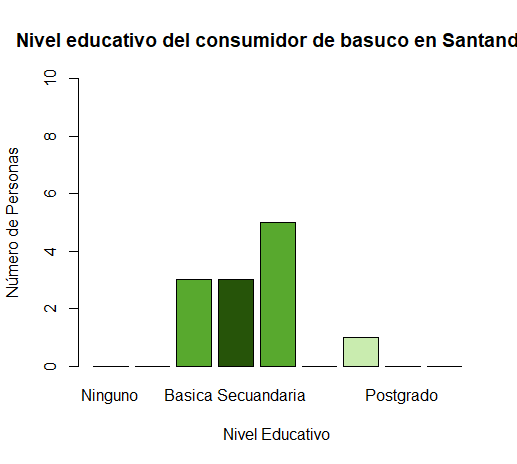
\includegraphics{images/basuco educacion santander.png}

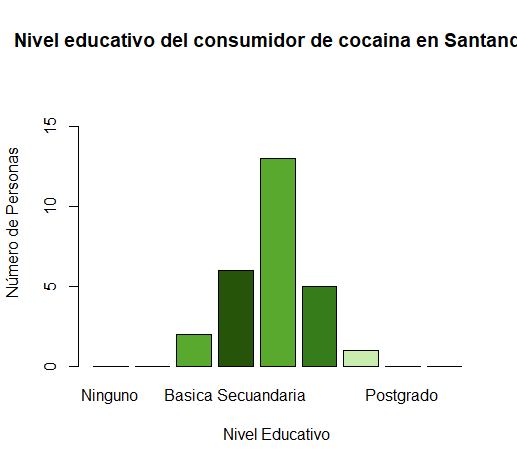
\includegraphics{images/cocaina educacion santander.png}

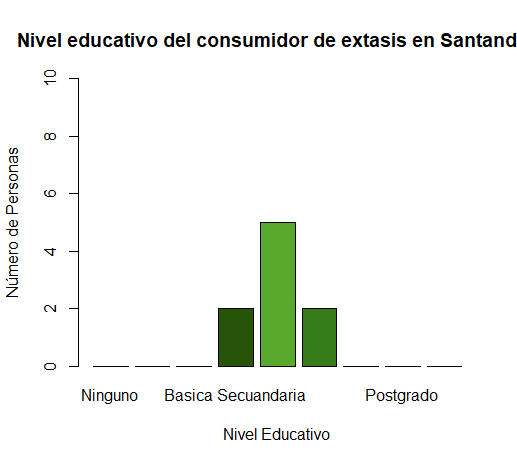
\includegraphics{images/extasis educacion santander.png}

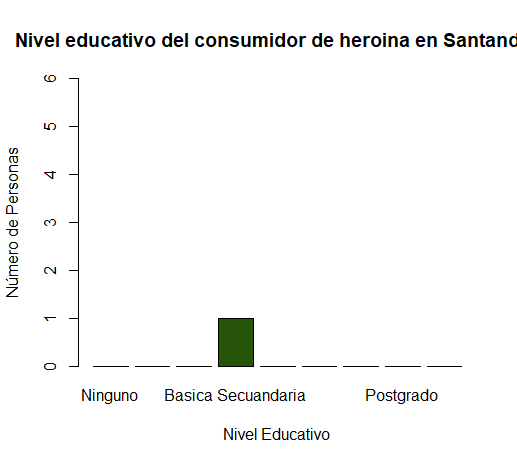
\includegraphics{images/heroina educacion santander.png}

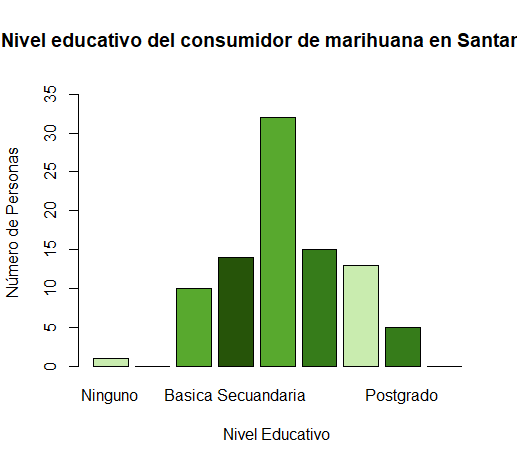
\includegraphics{images/marihuana eduacion santander.png}

Para el analisis anterior se siguio la sisguiente rutina:

Mostrar/Ocultar Código

\begin{Shaded}
\begin{Highlighting}[]
\NormalTok{reporte\_neducativo}\OtherTok{\textless{}{-}} \ControlFlowTok{function}\NormalTok{(data, columna, valores, etiquetas, nombre\_consumo, departamento, titulo\_grafico) \{}
\NormalTok{  cuentas }\OtherTok{\textless{}{-}} \FunctionTok{c}\NormalTok{()}
  
  \ControlFlowTok{for}\NormalTok{ (i }\ControlFlowTok{in} \FunctionTok{seq\_along}\NormalTok{(valores)) \{}
\NormalTok{    valor }\OtherTok{\textless{}{-}}\NormalTok{ valores[i]}
\NormalTok{    cuenta }\OtherTok{\textless{}{-}} \FunctionTok{sum}\NormalTok{(data[[columna]] }\SpecialCharTok{==}\NormalTok{ valor)}
\NormalTok{    cuentas }\OtherTok{\textless{}{-}} \FunctionTok{c}\NormalTok{(cuentas, cuenta)}
    
    \FunctionTok{cat}\NormalTok{(}\FunctionTok{sprintf}\NormalTok{(}
      \StringTok{"Personas que consumen \%s y tienen nivel educativo \%s en \%s: \%s}\SpecialCharTok{\textbackslash{}n}\StringTok{"}\NormalTok{, }
\NormalTok{      nombre\_consumo, etiquetas[i], departamento, cuenta}
\NormalTok{    ))}
\NormalTok{  \}}
  
  \CommentTok{\# Generar el gráfico}
  \FunctionTok{barplot}\NormalTok{(}
\NormalTok{    cuentas,}
    \AttributeTok{names.arg =}\NormalTok{ etiquetas,}
    \AttributeTok{col =} \FunctionTok{c}\NormalTok{(}\StringTok{"\#c9ecaf"}\NormalTok{, }\StringTok{"\#367c1a"}\NormalTok{, }\StringTok{"\#58a92e"}\NormalTok{, }\StringTok{"\#265409"}\NormalTok{, }\StringTok{"\#58a92e"}\NormalTok{, }\StringTok{"\#367c1a"}\NormalTok{, }\StringTok{"\#c9ecaf"}\NormalTok{, }\StringTok{"\#367c1a"}\NormalTok{, }\StringTok{"\#58a92e"}\NormalTok{),}
    \AttributeTok{main =} \FunctionTok{sprintf}\NormalTok{(}\StringTok{"\%s en \%s"}\NormalTok{, titulo\_grafico, departamento),}
    \AttributeTok{xlab =} \StringTok{"Nivel Educativo"}\NormalTok{,}
    \AttributeTok{ylab =} \StringTok{"Número de Personas"}\NormalTok{,}
    \AttributeTok{ylim =} \FunctionTok{c}\NormalTok{(}\DecValTok{0}\NormalTok{, }\FunctionTok{max}\NormalTok{(cuentas) }\SpecialCharTok{+} \DecValTok{5}\NormalTok{)}
\NormalTok{  )}
\NormalTok{\}}

\FunctionTok{reporte\_neducativo}\NormalTok{(}
  \AttributeTok{data =}\NormalTok{ santander\_basuco,}
  \AttributeTok{columna =} \StringTok{"D2\_05"}\NormalTok{,}
  \AttributeTok{valores =} \FunctionTok{c}\NormalTok{(}\StringTok{"1"}\NormalTok{, }\StringTok{"2"}\NormalTok{, }\StringTok{"3"}\NormalTok{, }\StringTok{"4"}\NormalTok{, }\StringTok{"5"}\NormalTok{,}\StringTok{"6"}\NormalTok{, }\StringTok{"7"}\NormalTok{, }\StringTok{"8"}\NormalTok{, }\StringTok{"9"}\NormalTok{),}
  \AttributeTok{etiquetas =} \FunctionTok{c}\NormalTok{(}\StringTok{"Ninguno"}\NormalTok{, }\StringTok{"Preescolar"}\NormalTok{, }\StringTok{"Basica Primaria"}\NormalTok{, }\StringTok{"Basica Secuandaria"}\NormalTok{, }\StringTok{"Media"}\NormalTok{, }\StringTok{"Técnica/Tecnologica"}\NormalTok{, }\StringTok{"Universitaria"}\NormalTok{, }\StringTok{"Postgrado"}\NormalTok{, }\StringTok{"No sabe/informa"}\NormalTok{),}
  \AttributeTok{nombre\_consumo =} \StringTok{"basuco"}\NormalTok{,}
  \AttributeTok{departamento =} \StringTok{"Santander"}\NormalTok{,}
  \AttributeTok{titulo\_grafico =} \StringTok{"Nivel educativo del consumidor de basuco"}
\NormalTok{)}

\FunctionTok{reporte\_neducativo}\NormalTok{(}
  \AttributeTok{data =}\NormalTok{ santander\_cocaina,}
  \AttributeTok{columna =} \StringTok{"D2\_05"}\NormalTok{,}
  \AttributeTok{valores =} \FunctionTok{c}\NormalTok{(}\StringTok{"1"}\NormalTok{, }\StringTok{"2"}\NormalTok{, }\StringTok{"3"}\NormalTok{, }\StringTok{"4"}\NormalTok{, }\StringTok{"5"}\NormalTok{,}\StringTok{"6"}\NormalTok{, }\StringTok{"7"}\NormalTok{, }\StringTok{"8"}\NormalTok{, }\StringTok{"9"}\NormalTok{),}
  \AttributeTok{etiquetas =} \FunctionTok{c}\NormalTok{(}\StringTok{"Ninguno"}\NormalTok{, }\StringTok{"Preescolar"}\NormalTok{, }\StringTok{"Basica Primaria"}\NormalTok{, }\StringTok{"Basica Secuandaria"}\NormalTok{, }\StringTok{"Media"}\NormalTok{, }\StringTok{"Técnica/Tecnologica"}\NormalTok{, }\StringTok{"Universitaria"}\NormalTok{, }\StringTok{"Postgrado"}\NormalTok{, }\StringTok{"No sabe/informa"}\NormalTok{),}
  \AttributeTok{nombre\_consumo =} \StringTok{"cocaina"}\NormalTok{,}
  \AttributeTok{departamento =} \StringTok{"Santander"}\NormalTok{,}
  \AttributeTok{titulo\_grafico =} \StringTok{"Nivel educativo del consumidor de cocaina"}
\NormalTok{)}

\FunctionTok{reporte\_neducativo}\NormalTok{(}
  \AttributeTok{data =}\NormalTok{ santander\_extasis,}
  \AttributeTok{columna =} \StringTok{"D2\_05"}\NormalTok{,}
  \AttributeTok{valores =} \FunctionTok{c}\NormalTok{(}\StringTok{"1"}\NormalTok{, }\StringTok{"2"}\NormalTok{, }\StringTok{"3"}\NormalTok{, }\StringTok{"4"}\NormalTok{, }\StringTok{"5"}\NormalTok{,}\StringTok{"6"}\NormalTok{, }\StringTok{"7"}\NormalTok{, }\StringTok{"8"}\NormalTok{, }\StringTok{"9"}\NormalTok{),}
  \AttributeTok{etiquetas =} \FunctionTok{c}\NormalTok{(}\StringTok{"Ninguno"}\NormalTok{, }\StringTok{"Preescolar"}\NormalTok{, }\StringTok{"Basica Primaria"}\NormalTok{, }\StringTok{"Basica Secuandaria"}\NormalTok{, }\StringTok{"Media"}\NormalTok{, }\StringTok{"Técnica/Tecnologica"}\NormalTok{, }\StringTok{"Universitaria"}\NormalTok{, }\StringTok{"Postgrado"}\NormalTok{, }\StringTok{"No sabe/informa"}\NormalTok{),}
  \AttributeTok{nombre\_consumo =} \StringTok{"extasis"}\NormalTok{,}
  \AttributeTok{departamento =} \StringTok{"Santander"}\NormalTok{,}
  \AttributeTok{titulo\_grafico =} \StringTok{"Nivel educativo del consumidor de extasis"}
\NormalTok{)}

\FunctionTok{reporte\_neducativo}\NormalTok{(}
  \AttributeTok{data =}\NormalTok{ santander\_heroina,}
  \AttributeTok{columna =} \StringTok{"D2\_05"}\NormalTok{,}
  \AttributeTok{valores =} \FunctionTok{c}\NormalTok{(}\StringTok{"1"}\NormalTok{, }\StringTok{"2"}\NormalTok{, }\StringTok{"3"}\NormalTok{, }\StringTok{"4"}\NormalTok{, }\StringTok{"5"}\NormalTok{,}\StringTok{"6"}\NormalTok{, }\StringTok{"7"}\NormalTok{, }\StringTok{"8"}\NormalTok{, }\StringTok{"9"}\NormalTok{),}
  \AttributeTok{etiquetas =} \FunctionTok{c}\NormalTok{(}\StringTok{"Ninguno"}\NormalTok{, }\StringTok{"Preescolar"}\NormalTok{, }\StringTok{"Basica Primaria"}\NormalTok{, }\StringTok{"Basica Secuandaria"}\NormalTok{, }\StringTok{"Media"}\NormalTok{, }\StringTok{"Técnica/Tecnologica"}\NormalTok{, }\StringTok{"Universitaria"}\NormalTok{, }\StringTok{"Postgrado"}\NormalTok{, }\StringTok{"No sabe/informa"}\NormalTok{),}
  \AttributeTok{nombre\_consumo =} \StringTok{"heroina"}\NormalTok{,}
  \AttributeTok{departamento =} \StringTok{"Santander"}\NormalTok{,}
  \AttributeTok{titulo\_grafico =} \StringTok{"Nivel educativo del consumidor de heroina"}
\NormalTok{)}

\FunctionTok{reporte\_neducativo}\NormalTok{(}
  \AttributeTok{data =}\NormalTok{ santander\_marihuana,}
  \AttributeTok{columna =} \StringTok{"D2\_05"}\NormalTok{,}
  \AttributeTok{valores =} \FunctionTok{c}\NormalTok{(}\StringTok{"1"}\NormalTok{, }\StringTok{"2"}\NormalTok{, }\StringTok{"3"}\NormalTok{, }\StringTok{"4"}\NormalTok{, }\StringTok{"5"}\NormalTok{,}\StringTok{"6"}\NormalTok{, }\StringTok{"7"}\NormalTok{, }\StringTok{"8"}\NormalTok{, }\StringTok{"9"}\NormalTok{),}
  \AttributeTok{etiquetas =} \FunctionTok{c}\NormalTok{(}\StringTok{"Ninguno"}\NormalTok{, }\StringTok{"Preescolar"}\NormalTok{, }\StringTok{"Basica Primaria"}\NormalTok{, }\StringTok{"Basica Secuandaria"}\NormalTok{, }\StringTok{"Media"}\NormalTok{, }\StringTok{"Técnica/Tecnologica"}\NormalTok{, }\StringTok{"Universitaria"}\NormalTok{, }\StringTok{"Postgrado"}\NormalTok{, }\StringTok{"No sabe/informa"}\NormalTok{),}
  \AttributeTok{nombre\_consumo =} \StringTok{"marihuana"}\NormalTok{,}
  \AttributeTok{departamento =} \StringTok{"Santander"}\NormalTok{,}
  \AttributeTok{titulo\_grafico =} \StringTok{"Nivel educativo del consumidor de marihuana"}
\NormalTok{)}
\end{Highlighting}
\end{Shaded}

\begin{enumerate}
\def\labelenumi{\arabic{enumi}.}
\setcounter{enumi}{3}
\tightlist
\item
  Consumo y por genero:
\end{enumerate}

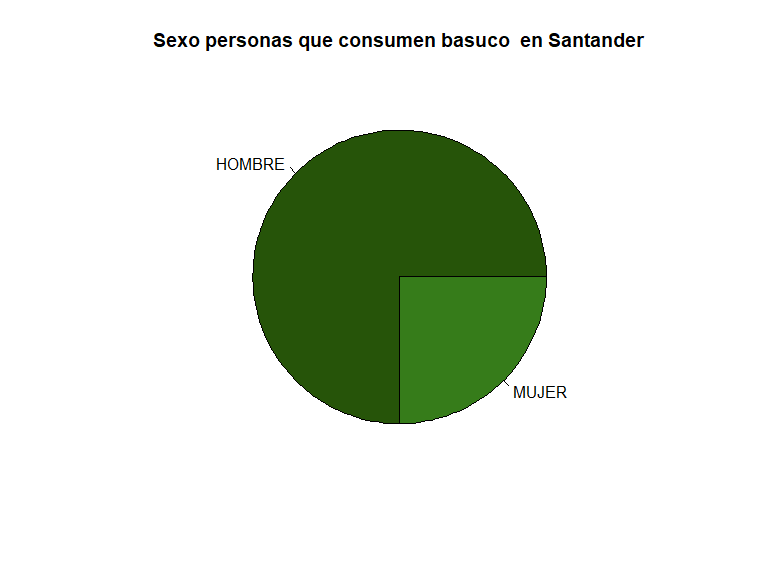
\includegraphics{images/basuco S santander.png}

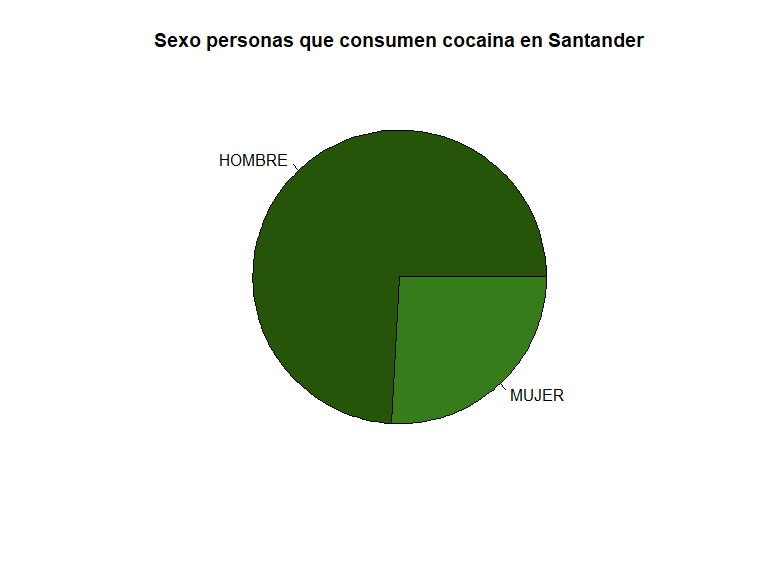
\includegraphics{images/cocaina S santander.png}

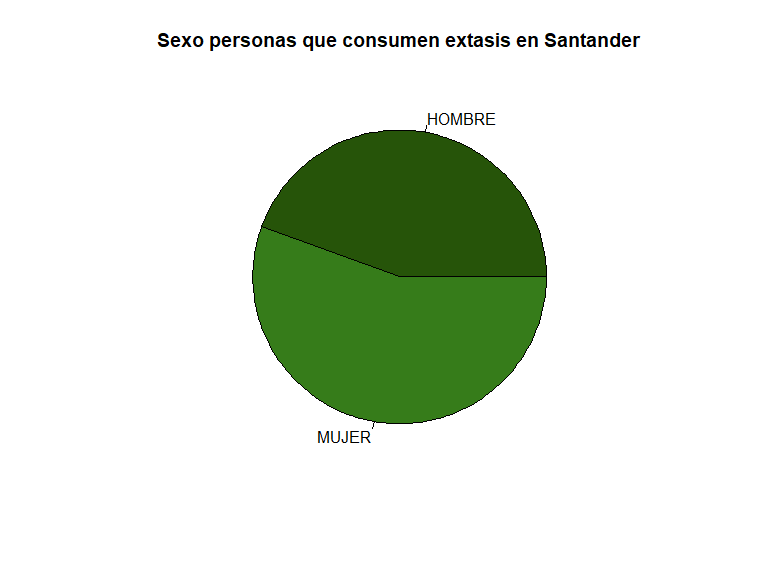
\includegraphics{images/extasis S santander.png}

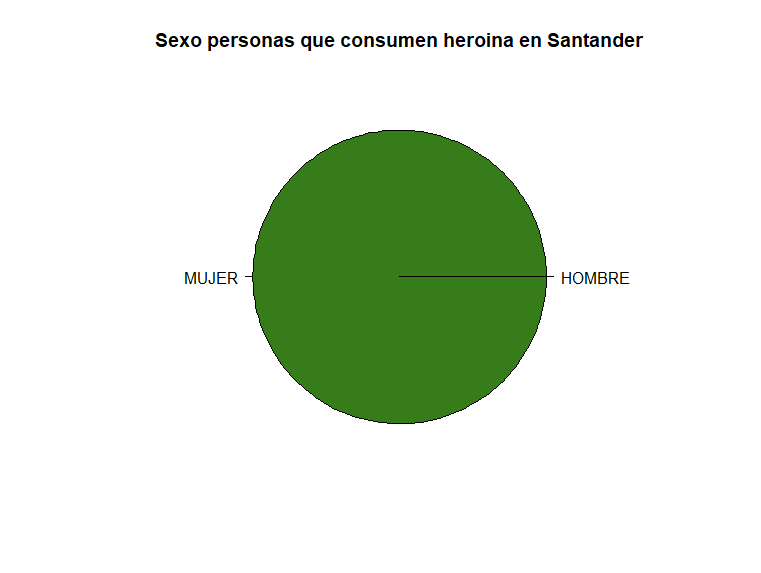
\includegraphics{images/heroina S santander.png}

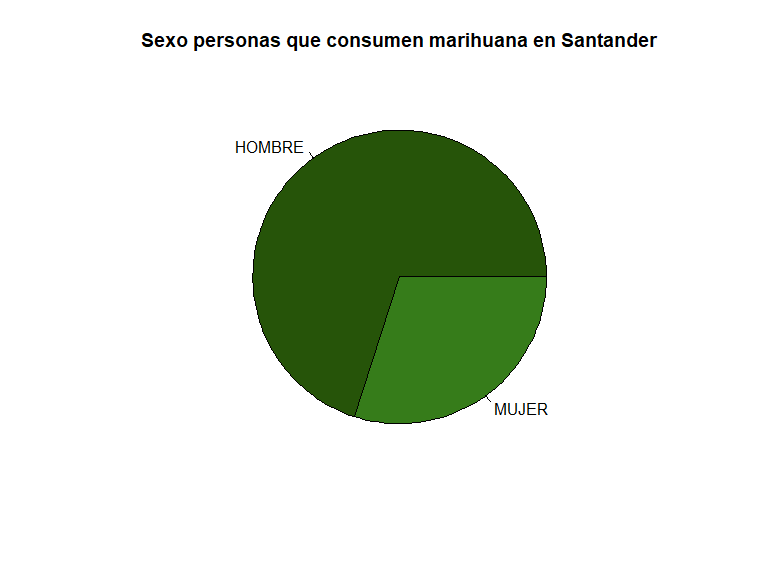
\includegraphics{images/marihuana S santander.png}

Para este analisis se siguio la siguiente rutina:

Mostrar/Ocultar Código

\begin{Shaded}
\begin{Highlighting}[]

\NormalTok{columna }\OtherTok{\textless{}{-}} \StringTok{"SEXO"}
\NormalTok{valores}\OtherTok{\textless{}{-}}\FunctionTok{c}\NormalTok{(}\StringTok{"1"}\NormalTok{, }\StringTok{"2"}\NormalTok{)}
\NormalTok{etiquetas }\OtherTok{\textless{}{-}} \FunctionTok{c}\NormalTok{(}
  \StringTok{"HOMBRE"}\NormalTok{,}
  \StringTok{"MUJER"}
\NormalTok{)}
\NormalTok{columna }\OtherTok{\textless{}{-}} \StringTok{"SEXO"}
\NormalTok{cuentas }\OtherTok{\textless{}{-}} \FunctionTok{c}\NormalTok{()}

\ControlFlowTok{for}\NormalTok{ (valor }\ControlFlowTok{in}\NormalTok{ valores) \{}
\NormalTok{  cuenta }\OtherTok{\textless{}{-}} \FunctionTok{sum}\NormalTok{(santander\_basuco[[columna]] }\SpecialCharTok{==}\NormalTok{ valor)}
\NormalTok{  cuentas }\OtherTok{\textless{}{-}} \FunctionTok{c}\NormalTok{(cuentas, cuenta)  }\CommentTok{\# Agregar cada cuenta al vector}
  
  \ControlFlowTok{if}\NormalTok{ (valor }\SpecialCharTok{==} \StringTok{"1"}\NormalTok{) \{}
    \FunctionTok{cat}\NormalTok{(}\FunctionTok{sprintf}\NormalTok{(}\StringTok{"Hombres que consumen:: \%s}\SpecialCharTok{\textbackslash{}n}\StringTok{"}\NormalTok{, cuenta))}
\NormalTok{  \} }\ControlFlowTok{else} \ControlFlowTok{if}\NormalTok{ (valor }\SpecialCharTok{==} \StringTok{"2"}\NormalTok{) \{}
    \FunctionTok{cat}\NormalTok{(}\FunctionTok{sprintf}\NormalTok{(}\StringTok{"Mujeres que consumen:: \%s}\SpecialCharTok{\textbackslash{}n}\StringTok{"}\NormalTok{, cuenta))}
\NormalTok{  \}}
\NormalTok{\}}

\FunctionTok{pie}\NormalTok{(}
\NormalTok{  cuentas,}
  \AttributeTok{labels =}\NormalTok{ etiquetas,}
  \AttributeTok{main =} \StringTok{"Sexo personas que consumen basuco  en Santander"}\NormalTok{,}
  \AttributeTok{col =} \FunctionTok{c}\NormalTok{(}\StringTok{"\#265409"}\NormalTok{, }\StringTok{"\#367c1a"}\NormalTok{)}
\NormalTok{)}

\CommentTok{\#Sexo de los consumidores cocaina }
\NormalTok{columna }\OtherTok{\textless{}{-}} \StringTok{"SEXO"}
\NormalTok{cuentas }\OtherTok{\textless{}{-}} \FunctionTok{c}\NormalTok{()}

\ControlFlowTok{for}\NormalTok{ (valor }\ControlFlowTok{in}\NormalTok{ valores) \{}
\NormalTok{  cuenta }\OtherTok{\textless{}{-}} \FunctionTok{sum}\NormalTok{(santander\_cocaina[[columna]] }\SpecialCharTok{==}\NormalTok{ valor)}
\NormalTok{  cuentas }\OtherTok{\textless{}{-}} \FunctionTok{c}\NormalTok{(cuentas, cuenta)  }\CommentTok{\# Agregar cada cuenta al vector}
  
  \ControlFlowTok{if}\NormalTok{ (valor }\SpecialCharTok{==} \StringTok{"1"}\NormalTok{) \{}
    \FunctionTok{cat}\NormalTok{(}\FunctionTok{sprintf}\NormalTok{(}\StringTok{"Hombres que consumen:: \%s}\SpecialCharTok{\textbackslash{}n}\StringTok{"}\NormalTok{, cuenta))}
\NormalTok{  \} }\ControlFlowTok{else} \ControlFlowTok{if}\NormalTok{ (valor }\SpecialCharTok{==} \StringTok{"2"}\NormalTok{) \{}
    \FunctionTok{cat}\NormalTok{(}\FunctionTok{sprintf}\NormalTok{(}\StringTok{"Mujeres que consumen:: \%s}\SpecialCharTok{\textbackslash{}n}\StringTok{"}\NormalTok{, cuenta))}
\NormalTok{  \}}
\NormalTok{\}}

\FunctionTok{pie}\NormalTok{(}
\NormalTok{  cuentas,}
  \AttributeTok{labels =}\NormalTok{ etiquetas,}
  \AttributeTok{main =} \StringTok{"Sexo personas que consumen cocaina en Santander"}\NormalTok{,}
  \AttributeTok{col =} \FunctionTok{c}\NormalTok{(}\StringTok{"\#265409"}\NormalTok{, }\StringTok{"\#367c1a"}\NormalTok{)}
\NormalTok{)}


\CommentTok{\#Sexo de los consumidores extasis }
\NormalTok{columna }\OtherTok{\textless{}{-}} \StringTok{"SEXO"}
\NormalTok{cuentas }\OtherTok{\textless{}{-}} \FunctionTok{c}\NormalTok{()}

\ControlFlowTok{for}\NormalTok{ (valor }\ControlFlowTok{in}\NormalTok{ valores) \{}
\NormalTok{  cuenta }\OtherTok{\textless{}{-}} \FunctionTok{sum}\NormalTok{(santander\_extasis[[columna]] }\SpecialCharTok{==}\NormalTok{ valor)}
\NormalTok{  cuentas }\OtherTok{\textless{}{-}} \FunctionTok{c}\NormalTok{(cuentas, cuenta)  }\CommentTok{\# Agregar cada cuenta al vector}
  
  \ControlFlowTok{if}\NormalTok{ (valor }\SpecialCharTok{==} \StringTok{"1"}\NormalTok{) \{}
    \FunctionTok{cat}\NormalTok{(}\FunctionTok{sprintf}\NormalTok{(}\StringTok{"Hombres que consumen:: \%s}\SpecialCharTok{\textbackslash{}n}\StringTok{"}\NormalTok{, cuenta))}
\NormalTok{  \} }\ControlFlowTok{else} \ControlFlowTok{if}\NormalTok{ (valor }\SpecialCharTok{==} \StringTok{"2"}\NormalTok{) \{}
    \FunctionTok{cat}\NormalTok{(}\FunctionTok{sprintf}\NormalTok{(}\StringTok{"Mujeres que consumen:: \%s}\SpecialCharTok{\textbackslash{}n}\StringTok{"}\NormalTok{, cuenta))}
\NormalTok{  \}}
\NormalTok{\}}

\FunctionTok{pie}\NormalTok{(}
\NormalTok{  cuentas,}
  \AttributeTok{labels =}\NormalTok{ etiquetas,}
  \AttributeTok{main =} \StringTok{"Sexo personas que consumen extasis en Santander"}\NormalTok{,}
  \AttributeTok{col =} \FunctionTok{c}\NormalTok{(}\StringTok{"\#265409"}\NormalTok{, }\StringTok{"\#367c1a"}\NormalTok{)}
\NormalTok{)}

\CommentTok{\#Sexo de los consumidores heroina }
\NormalTok{columna }\OtherTok{\textless{}{-}} \StringTok{"SEXO"}
\NormalTok{cuentas }\OtherTok{\textless{}{-}} \FunctionTok{c}\NormalTok{()}

\ControlFlowTok{for}\NormalTok{ (valor }\ControlFlowTok{in}\NormalTok{ valores) \{}
\NormalTok{  cuenta }\OtherTok{\textless{}{-}} \FunctionTok{sum}\NormalTok{(santander\_heroina[[columna]] }\SpecialCharTok{==}\NormalTok{ valor)}
\NormalTok{  cuentas }\OtherTok{\textless{}{-}} \FunctionTok{c}\NormalTok{(cuentas, cuenta)  }\CommentTok{\# Agregar cada cuenta al vector}
  
  \ControlFlowTok{if}\NormalTok{ (valor }\SpecialCharTok{==} \StringTok{"1"}\NormalTok{) \{}
    \FunctionTok{cat}\NormalTok{(}\FunctionTok{sprintf}\NormalTok{(}\StringTok{"Hombres que consumen:: \%s}\SpecialCharTok{\textbackslash{}n}\StringTok{"}\NormalTok{, cuenta))}
\NormalTok{  \} }\ControlFlowTok{else} \ControlFlowTok{if}\NormalTok{ (valor }\SpecialCharTok{==} \StringTok{"2"}\NormalTok{) \{}
    \FunctionTok{cat}\NormalTok{(}\FunctionTok{sprintf}\NormalTok{(}\StringTok{"Mujeres que consumen:: \%s}\SpecialCharTok{\textbackslash{}n}\StringTok{"}\NormalTok{, cuenta))}
\NormalTok{  \}}
\NormalTok{\}}

\FunctionTok{pie}\NormalTok{(}
\NormalTok{  cuentas,}
  \AttributeTok{labels =}\NormalTok{ etiquetas,}
  \AttributeTok{main =} \StringTok{"Sexo personas que consumen heroina en Santander"}\NormalTok{,}
  \AttributeTok{col =} \FunctionTok{c}\NormalTok{(}\StringTok{"\#265409"}\NormalTok{, }\StringTok{"\#367c1a"}\NormalTok{)}
\NormalTok{)}


\CommentTok{\#Sexo de los consumidores marihuana }
\NormalTok{columna }\OtherTok{\textless{}{-}} \StringTok{"SEXO"}
\NormalTok{cuentas }\OtherTok{\textless{}{-}} \FunctionTok{c}\NormalTok{()}

\ControlFlowTok{for}\NormalTok{ (valor }\ControlFlowTok{in}\NormalTok{ valores) \{}
\NormalTok{  cuenta }\OtherTok{\textless{}{-}} \FunctionTok{sum}\NormalTok{(santander\_marihuana[[columna]] }\SpecialCharTok{==}\NormalTok{ valor)}
\NormalTok{  cuentas }\OtherTok{\textless{}{-}} \FunctionTok{c}\NormalTok{(cuentas, cuenta)  }\CommentTok{\# Agregar cada cuenta al vector}
  
  \ControlFlowTok{if}\NormalTok{ (valor }\SpecialCharTok{==} \StringTok{"1"}\NormalTok{) \{}
    \FunctionTok{cat}\NormalTok{(}\FunctionTok{sprintf}\NormalTok{(}\StringTok{"Hombres que consumen:: \%s}\SpecialCharTok{\textbackslash{}n}\StringTok{"}\NormalTok{, cuenta))}
\NormalTok{  \} }\ControlFlowTok{else} \ControlFlowTok{if}\NormalTok{ (valor }\SpecialCharTok{==} \StringTok{"2"}\NormalTok{) \{}
    \FunctionTok{cat}\NormalTok{(}\FunctionTok{sprintf}\NormalTok{(}\StringTok{"Mujeres que consumen:: \%s}\SpecialCharTok{\textbackslash{}n}\StringTok{"}\NormalTok{, cuenta))}
\NormalTok{  \}}
\NormalTok{\}}

\FunctionTok{pie}\NormalTok{(}
\NormalTok{  cuentas,}
  \AttributeTok{labels =}\NormalTok{ etiquetas,}
  \AttributeTok{main =} \StringTok{"Sexo personas que consumen marihuana en Santander"}\NormalTok{,}
  \AttributeTok{col =} \FunctionTok{c}\NormalTok{(}\StringTok{"\#265409"}\NormalTok{, }\StringTok{"\#367c1a"}\NormalTok{)}
\NormalTok{)}
\end{Highlighting}
\end{Shaded}

\begin{enumerate}
\def\labelenumi{\arabic{enumi}.}
\setcounter{enumi}{4}
\tightlist
\item
  Consumo y raices culturales:
\end{enumerate}

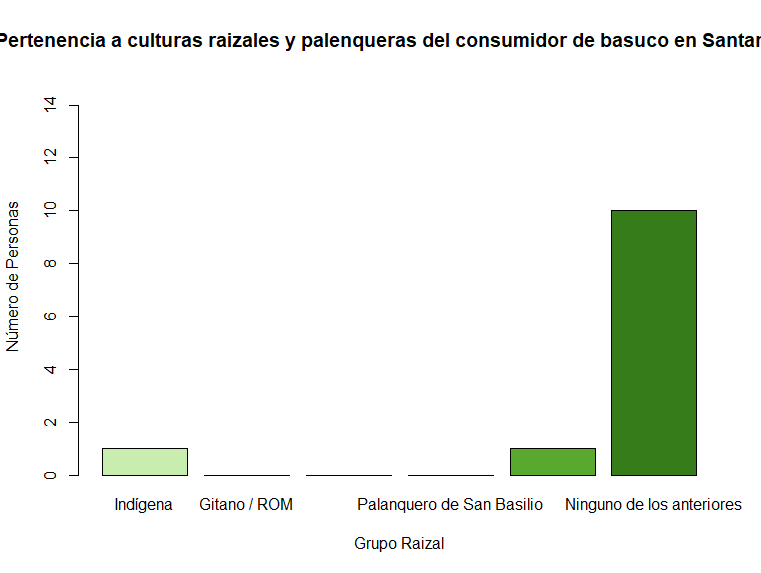
\includegraphics{images/basuco cultura santander.png}

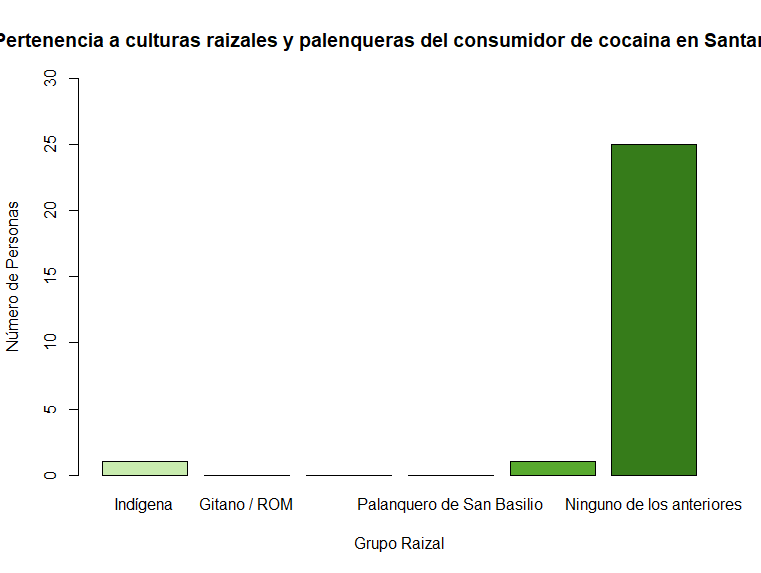
\includegraphics{images/cocaina cultura santander.png}

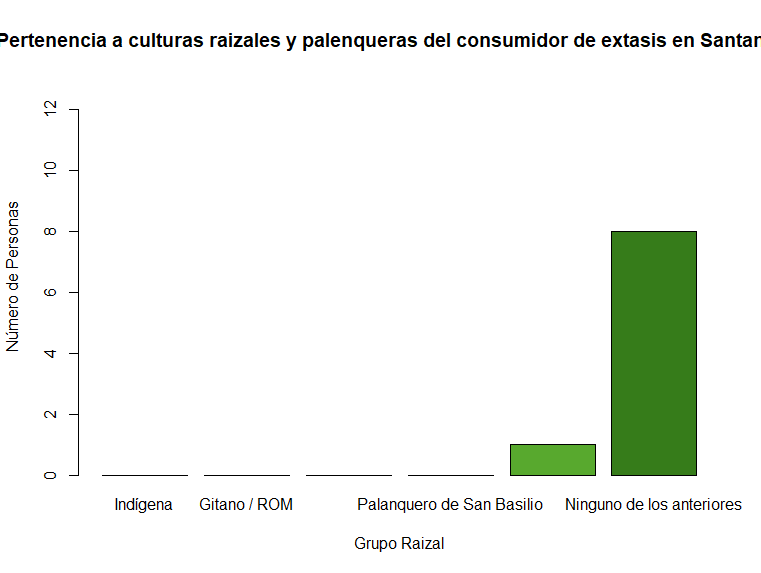
\includegraphics{images/extasis cultura santander.png}

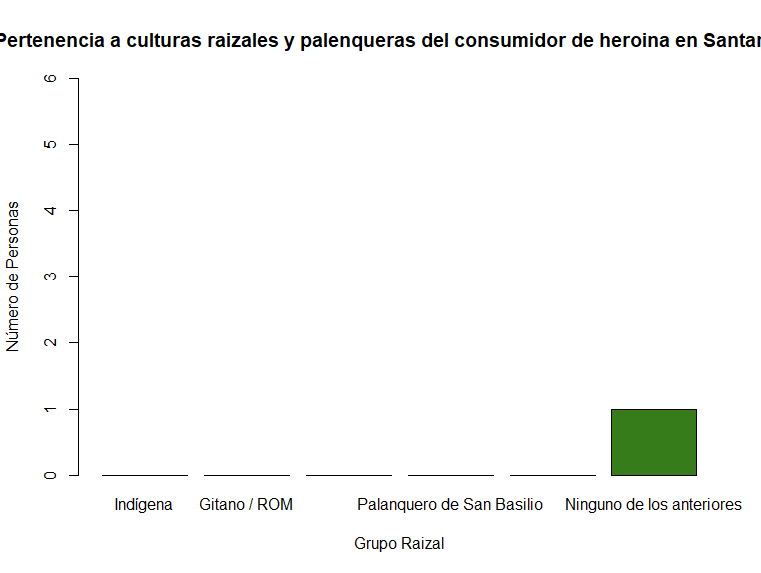
\includegraphics{images/heroina cultura santander.png}

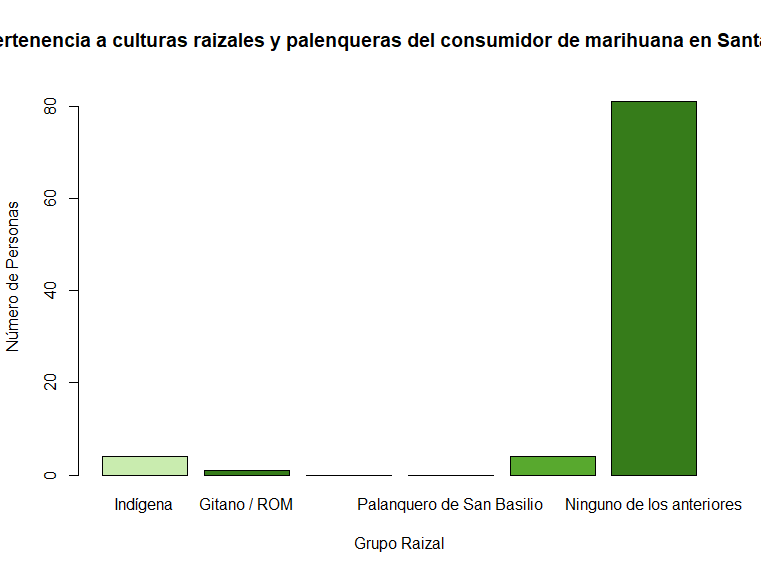
\includegraphics{images/marihuana cultura santander.png}

Para las graficas anteriores se siguio la siguiente rutina:

Mostrar/Ocultar Código

\begin{Shaded}
\begin{Highlighting}[]
\NormalTok{reporte\_raizal}\OtherTok{\textless{}{-}} \ControlFlowTok{function}\NormalTok{(data, columna, valores, etiquetas, nombre\_consumo, departamento, titulo\_grafico) \{}
\NormalTok{  cuentas }\OtherTok{\textless{}{-}} \FunctionTok{c}\NormalTok{()}
  
  \ControlFlowTok{for}\NormalTok{ (i }\ControlFlowTok{in} \FunctionTok{seq\_along}\NormalTok{(valores)) \{}
\NormalTok{    valor }\OtherTok{\textless{}{-}}\NormalTok{ valores[i]}
\NormalTok{    cuenta }\OtherTok{\textless{}{-}} \FunctionTok{sum}\NormalTok{(data[[columna]] }\SpecialCharTok{==}\NormalTok{ valor)}
\NormalTok{    cuentas }\OtherTok{\textless{}{-}} \FunctionTok{c}\NormalTok{(cuentas, cuenta)}
    
    \FunctionTok{cat}\NormalTok{(}\FunctionTok{sprintf}\NormalTok{(}
      \StringTok{"Personas que consumen \%s y pertenecen al grupo \%s en \%s: \%s}\SpecialCharTok{\textbackslash{}n}\StringTok{"}\NormalTok{, }
\NormalTok{      nombre\_consumo, etiquetas[i], departamento, cuenta}
\NormalTok{    ))}
\NormalTok{  \}}
  
  \CommentTok{\# Generar el gráfico}
  \FunctionTok{barplot}\NormalTok{(}
\NormalTok{    cuentas,}
    \AttributeTok{names.arg =}\NormalTok{ etiquetas,}
    \AttributeTok{col =} \FunctionTok{c}\NormalTok{(}\StringTok{"\#c9ecaf"}\NormalTok{, }\StringTok{"\#367c1a"}\NormalTok{, }\StringTok{"\#58a92e"}\NormalTok{, }\StringTok{"\#265409"}\NormalTok{, }\StringTok{"\#58a92e"}\NormalTok{, }\StringTok{"\#367c1a"}\NormalTok{),}
    \AttributeTok{main =} \FunctionTok{sprintf}\NormalTok{(}\StringTok{"\%s en \%s"}\NormalTok{, titulo\_grafico, departamento),}
    \AttributeTok{xlab =} \StringTok{"Grupo Raizal"}\NormalTok{,}
    \AttributeTok{ylab =} \StringTok{"Número de Personas"}\NormalTok{,}
    \AttributeTok{ylim =} \FunctionTok{c}\NormalTok{(}\DecValTok{0}\NormalTok{, }\FunctionTok{max}\NormalTok{(cuentas) }\SpecialCharTok{+} \DecValTok{5}\NormalTok{)}
\NormalTok{  )}
\NormalTok{\}}

\FunctionTok{reporte\_raizal}\NormalTok{(}
  \AttributeTok{data =}\NormalTok{ santander\_basuco,}
  \AttributeTok{columna =} \StringTok{"D2\_01"}\NormalTok{,}
  \AttributeTok{valores =} \FunctionTok{c}\NormalTok{(}\StringTok{"1"}\NormalTok{, }\StringTok{"2"}\NormalTok{, }\StringTok{"3"}\NormalTok{, }\StringTok{"4"}\NormalTok{, }\StringTok{"5"}\NormalTok{, }\StringTok{"9"}\NormalTok{),}
  \AttributeTok{etiquetas =} \FunctionTok{c}\NormalTok{(}\StringTok{"Indígena"}\NormalTok{, }\StringTok{"Gitano / ROM"}\NormalTok{, }\StringTok{"Raizal Isleño"}\NormalTok{, }\StringTok{"Palanquero de San Basilio"}\NormalTok{, }\StringTok{"Negro o afrocolombiano"}\NormalTok{, }\StringTok{"Ninguno de los anteriores"}\NormalTok{),}
  \AttributeTok{nombre\_consumo =} \StringTok{"basuco"}\NormalTok{,}
  \AttributeTok{departamento =} \StringTok{"Santander "}\NormalTok{,}
  \AttributeTok{titulo\_grafico =} \StringTok{"Pertenencia a culturas raizales y palenqueras del consumidor de basuco"}
\NormalTok{)}

\FunctionTok{reporte\_raizal}\NormalTok{(}
  \AttributeTok{data =}\NormalTok{ santander\_cocaina,}
  \AttributeTok{columna =} \StringTok{"D2\_01"}\NormalTok{,}
  \AttributeTok{valores =} \FunctionTok{c}\NormalTok{(}\StringTok{"1"}\NormalTok{, }\StringTok{"2"}\NormalTok{, }\StringTok{"3"}\NormalTok{, }\StringTok{"4"}\NormalTok{, }\StringTok{"5"}\NormalTok{, }\StringTok{"9"}\NormalTok{),}
  \AttributeTok{etiquetas =} \FunctionTok{c}\NormalTok{(}\StringTok{"Indígena"}\NormalTok{, }\StringTok{"Gitano / ROM"}\NormalTok{, }\StringTok{"Raizal Isleño"}\NormalTok{, }\StringTok{"Palanquero de San Basilio"}\NormalTok{, }\StringTok{"Negro o afrocolombiano"}\NormalTok{, }\StringTok{"Ninguno de los anteriores"}\NormalTok{),}
  \AttributeTok{nombre\_consumo =} \StringTok{"cocaina"}\NormalTok{,}
  \AttributeTok{departamento =} \StringTok{"Santander "}\NormalTok{,}
  \AttributeTok{titulo\_grafico =} \StringTok{"Pertenencia a culturas raizales y palenqueras del consumidor de cocaina"}
\NormalTok{)}

\FunctionTok{reporte\_raizal}\NormalTok{(}
  \AttributeTok{data =}\NormalTok{ santander\_extasis,}
  \AttributeTok{columna =} \StringTok{"D2\_01"}\NormalTok{,}
  \AttributeTok{valores =} \FunctionTok{c}\NormalTok{(}\StringTok{"1"}\NormalTok{, }\StringTok{"2"}\NormalTok{, }\StringTok{"3"}\NormalTok{, }\StringTok{"4"}\NormalTok{, }\StringTok{"5"}\NormalTok{, }\StringTok{"9"}\NormalTok{),}
  \AttributeTok{etiquetas =} \FunctionTok{c}\NormalTok{(}\StringTok{"Indígena"}\NormalTok{, }\StringTok{"Gitano / ROM"}\NormalTok{, }\StringTok{"Raizal Isleño"}\NormalTok{, }\StringTok{"Palanquero de San Basilio"}\NormalTok{, }\StringTok{"Negro o afrocolombiano"}\NormalTok{, }\StringTok{"Ninguno de los anteriores"}\NormalTok{),}
  \AttributeTok{nombre\_consumo =} \StringTok{"extasis"}\NormalTok{,}
  \AttributeTok{departamento =} \StringTok{"Santander "}\NormalTok{,}
  \AttributeTok{titulo\_grafico =} \StringTok{"Pertenencia a culturas raizales y palenqueras del consumidor de extasis"}
\NormalTok{)}

\FunctionTok{reporte\_raizal}\NormalTok{(}
  \AttributeTok{data =}\NormalTok{ santander\_heroina,}
  \AttributeTok{columna =} \StringTok{"D2\_01"}\NormalTok{,}
  \AttributeTok{valores =} \FunctionTok{c}\NormalTok{(}\StringTok{"1"}\NormalTok{, }\StringTok{"2"}\NormalTok{, }\StringTok{"3"}\NormalTok{, }\StringTok{"4"}\NormalTok{, }\StringTok{"5"}\NormalTok{, }\StringTok{"9"}\NormalTok{),}
  \AttributeTok{etiquetas =} \FunctionTok{c}\NormalTok{(}\StringTok{"Indígena"}\NormalTok{, }\StringTok{"Gitano / ROM"}\NormalTok{, }\StringTok{"Raizal Isleño"}\NormalTok{, }\StringTok{"Palanquero de San Basilio"}\NormalTok{, }\StringTok{"Negro o afrocolombiano"}\NormalTok{, }\StringTok{"Ninguno de los anteriores"}\NormalTok{),}
  \AttributeTok{nombre\_consumo =} \StringTok{"heroina"}\NormalTok{,}
  \AttributeTok{departamento =} \StringTok{"Santander "}\NormalTok{,}
  \AttributeTok{titulo\_grafico =} \StringTok{"Pertenencia a culturas raizales y palenqueras del consumidor de heroina"}
\NormalTok{)}

\FunctionTok{reporte\_raizal}\NormalTok{(}
  \AttributeTok{data =}\NormalTok{ santander\_marihuana,}
  \AttributeTok{columna =} \StringTok{"D2\_01"}\NormalTok{,}
  \AttributeTok{valores =} \FunctionTok{c}\NormalTok{(}\StringTok{"1"}\NormalTok{, }\StringTok{"2"}\NormalTok{, }\StringTok{"3"}\NormalTok{, }\StringTok{"4"}\NormalTok{, }\StringTok{"5"}\NormalTok{, }\StringTok{"9"}\NormalTok{),}
  \AttributeTok{etiquetas =} \FunctionTok{c}\NormalTok{(}\StringTok{"Indígena"}\NormalTok{, }\StringTok{"Gitano / ROM"}\NormalTok{, }\StringTok{"Raizal Isleño"}\NormalTok{, }\StringTok{"Palanquero de San Basilio"}\NormalTok{, }\StringTok{"Negro o afrocolombiano"}\NormalTok{, }\StringTok{"Ninguno de los anteriores"}\NormalTok{),}
  \AttributeTok{nombre\_consumo =} \StringTok{"marihuana"}\NormalTok{,}
  \AttributeTok{departamento =} \StringTok{"Santander "}\NormalTok{,}
  \AttributeTok{titulo\_grafico =} \StringTok{"Pertenencia a culturas raizales y palenqueras del consumidor de marihuana"}
\NormalTok{)}
\end{Highlighting}
\end{Shaded}

\begin{enumerate}
\def\labelenumi{\arabic{enumi}.}
\setcounter{enumi}{4}
\tightlist
\item
  Consumo y edad:
\end{enumerate}

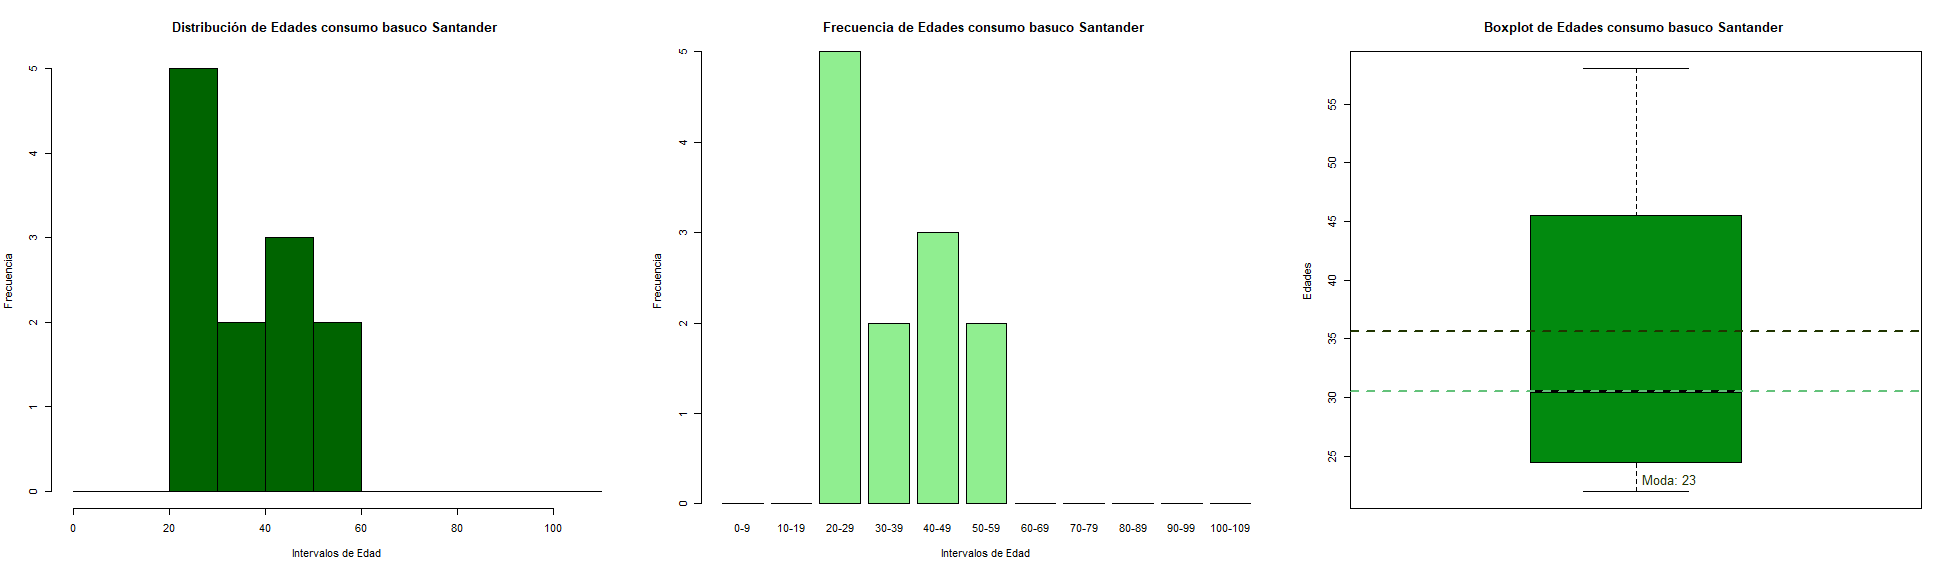
\includegraphics{images/basuco edad santander.png}

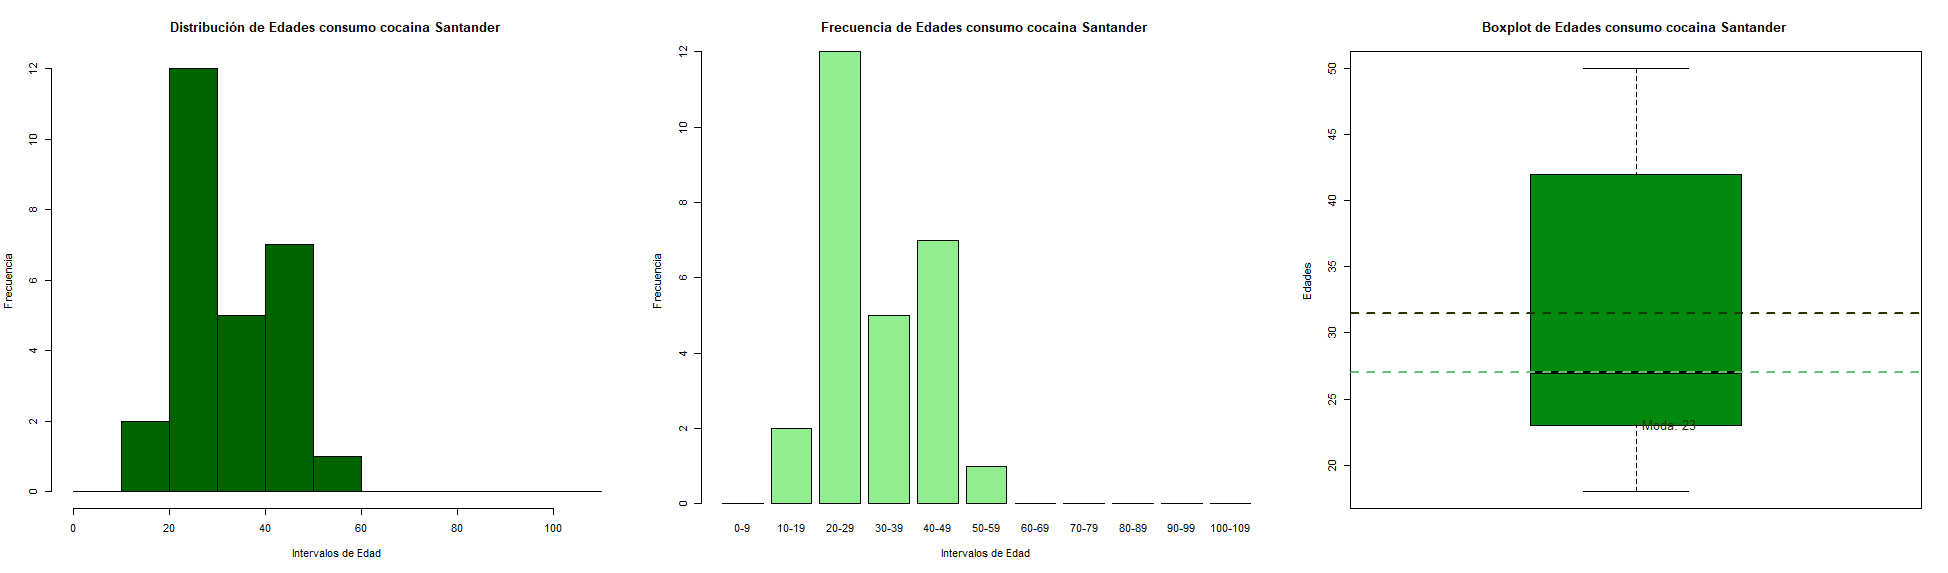
\includegraphics{images/cocaina edad santander.png}

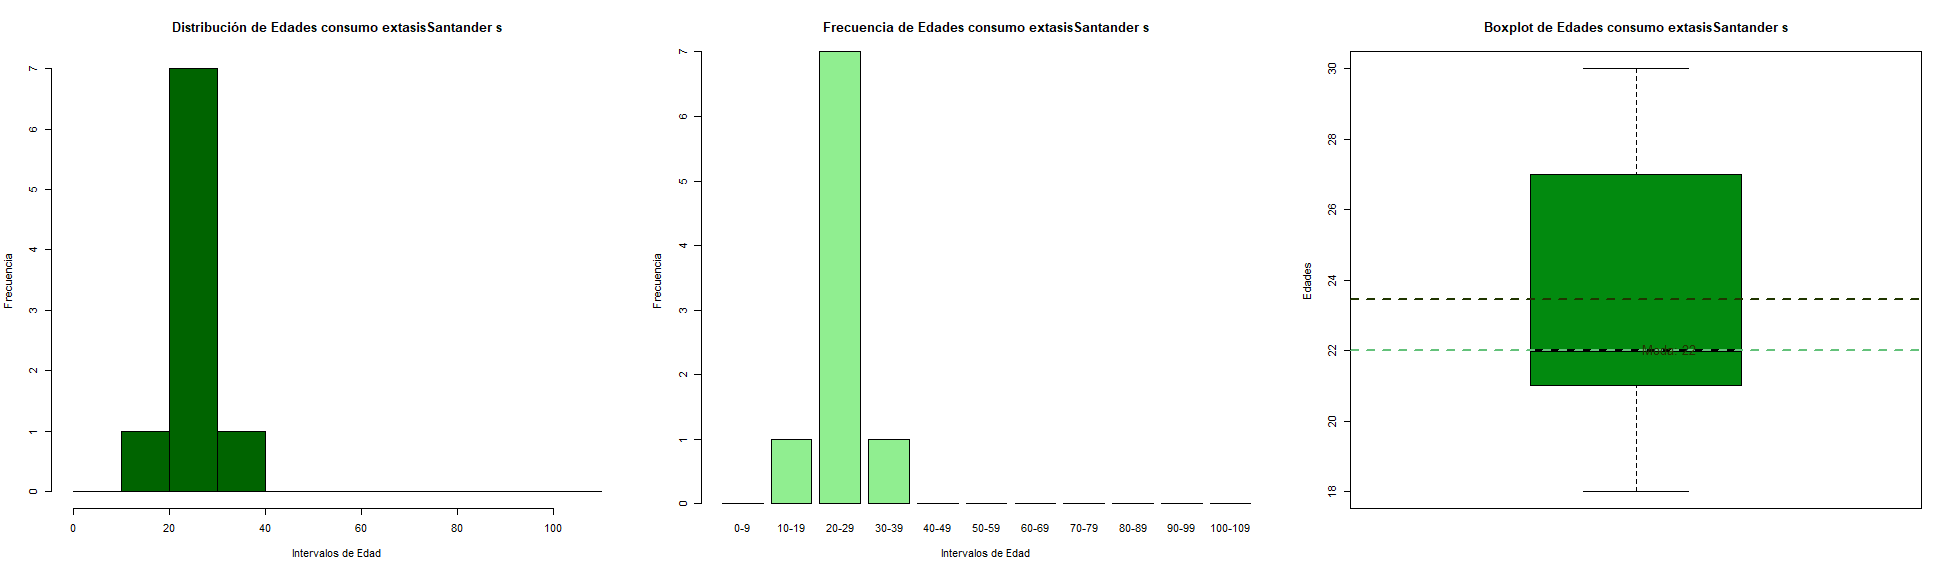
\includegraphics{images/extasis edad santander.png}

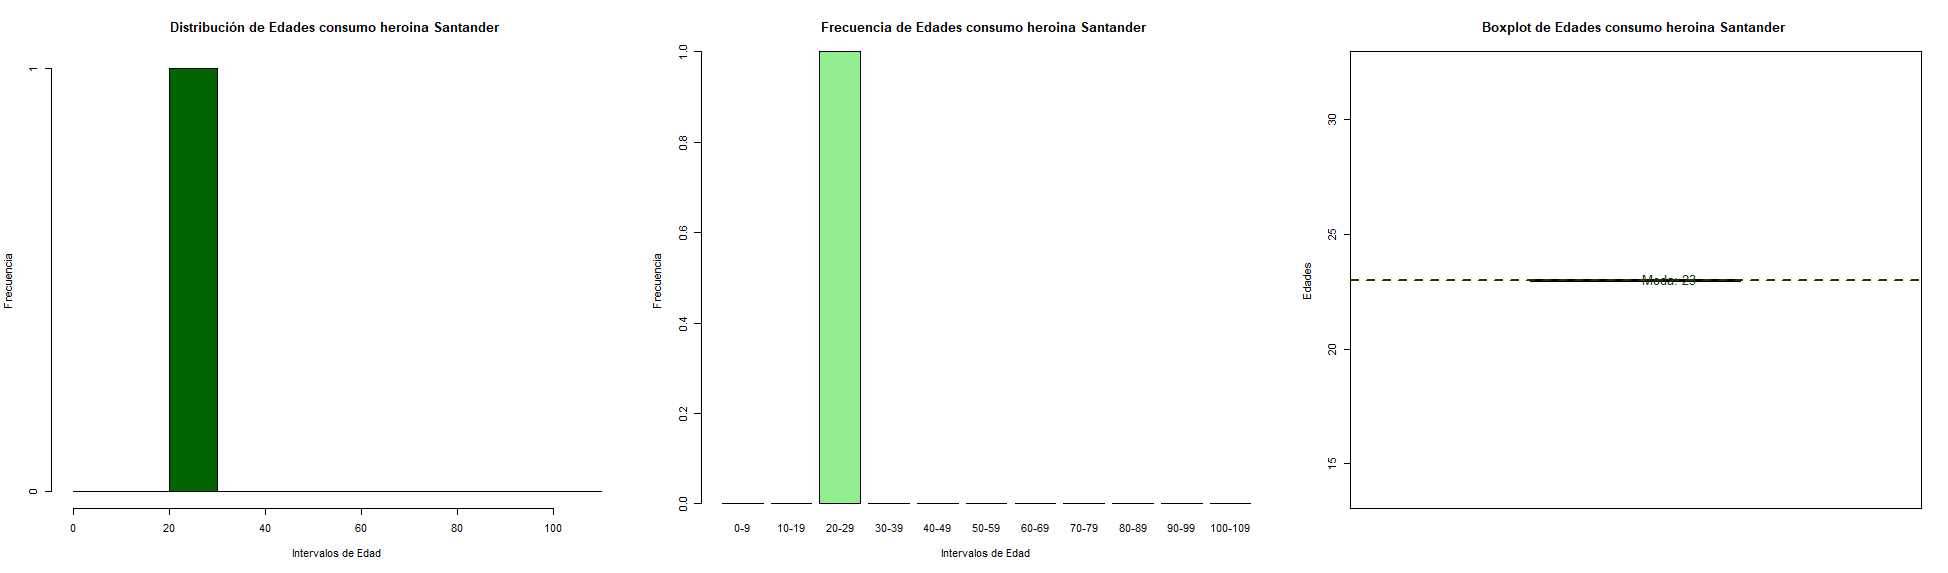
\includegraphics{images/heroina edad santander.png}

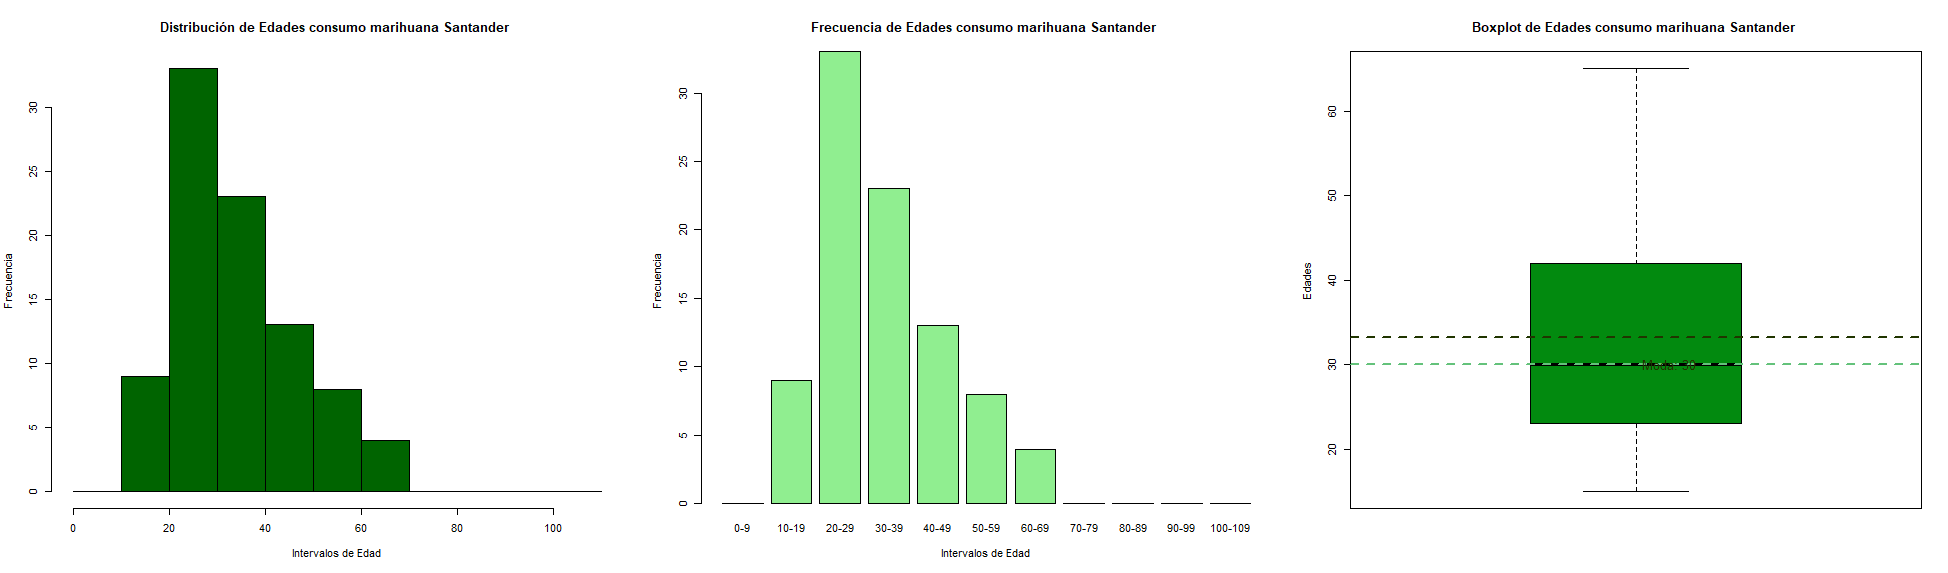
\includegraphics{images/marihuana edad santander.png}

Para las graficas de la edad se siguió la siguiente rutina:

Mostrar/Ocultar Código

\begin{Shaded}
\begin{Highlighting}[]
\NormalTok{analizar\_edades }\OtherTok{\textless{}{-}} \ControlFlowTok{function}\NormalTok{(data, columna, }\AttributeTok{nombre\_variable =} \StringTok{"Variable"}\NormalTok{, }\AttributeTok{intervalos\_breaks =} \ConstantTok{NULL}\NormalTok{) \{}
  \ControlFlowTok{if}\NormalTok{ (}\SpecialCharTok{!}\NormalTok{columna }\SpecialCharTok{\%in\%} \FunctionTok{names}\NormalTok{(data)) \{}
    \FunctionTok{stop}\NormalTok{(}\FunctionTok{sprintf}\NormalTok{(}\StringTok{"La columna \textquotesingle{}\%s\textquotesingle{} no existe en el dataset."}\NormalTok{, columna))}
\NormalTok{  \}}
  
\NormalTok{  edades }\OtherTok{\textless{}{-}} \FunctionTok{as.numeric}\NormalTok{(data[[columna]])}
  \ControlFlowTok{if}\NormalTok{ (}\FunctionTok{any}\NormalTok{(}\FunctionTok{is.na}\NormalTok{(edades))) \{}
    \FunctionTok{cat}\NormalTok{(}\StringTok{"Aviso: Se encontraron valores NA, que serán excluidos del análisis.}\SpecialCharTok{\textbackslash{}n}\StringTok{"}\NormalTok{)}
\NormalTok{  \}}
\NormalTok{  edades }\OtherTok{\textless{}{-}}\NormalTok{ edades[}\SpecialCharTok{!}\FunctionTok{is.na}\NormalTok{(edades)]}
  
  \CommentTok{\#Se indican los intervalos}
\NormalTok{  intervalos\_breaks }\OtherTok{=} \FunctionTok{c}\NormalTok{(}\DecValTok{0}\NormalTok{, }\DecValTok{10}\NormalTok{, }\DecValTok{20}\NormalTok{, }\DecValTok{30}\NormalTok{, }\DecValTok{40}\NormalTok{, }\DecValTok{50}\NormalTok{, }\DecValTok{60}\NormalTok{, }\DecValTok{70}\NormalTok{, }\DecValTok{80}\NormalTok{, }\DecValTok{90}\NormalTok{, }\DecValTok{100}\NormalTok{, }\DecValTok{110}\NormalTok{)}
  
  \CommentTok{\#Se calculan las medidas generales}
\NormalTok{  media\_general }\OtherTok{\textless{}{-}} \FunctionTok{mean}\NormalTok{(edades)}
\NormalTok{  mediana\_general }\OtherTok{\textless{}{-}} \FunctionTok{median}\NormalTok{(edades)}
\NormalTok{  desviacion\_general }\OtherTok{\textless{}{-}} \FunctionTok{sd}\NormalTok{(edades)}
\NormalTok{  sesgo }\OtherTok{\textless{}{-}} \FunctionTok{skewness}\NormalTok{(edades)}
\NormalTok{  curtosis }\OtherTok{\textless{}{-}} \FunctionTok{kurtosis}\NormalTok{(edades)}
  
  \CommentTok{\# Función para calcular la moda}
\NormalTok{  calcular\_moda }\OtherTok{\textless{}{-}} \ControlFlowTok{function}\NormalTok{(x) \{}
\NormalTok{    uniq\_x }\OtherTok{\textless{}{-}} \FunctionTok{unique}\NormalTok{(x)}
\NormalTok{    uniq\_x[}\FunctionTok{which.max}\NormalTok{(}\FunctionTok{tabulate}\NormalTok{(}\FunctionTok{match}\NormalTok{(x, uniq\_x)))]}
\NormalTok{  \}}
\NormalTok{  moda\_general }\OtherTok{\textless{}{-}} \FunctionTok{calcular\_moda}\NormalTok{(edades)}
  
  \CommentTok{\# Imprimir estadísticas generales}
  \FunctionTok{cat}\NormalTok{(}\FunctionTok{sprintf}\NormalTok{(}\StringTok{"Análisis de \%s}\SpecialCharTok{\textbackslash{}n}\StringTok{"}\NormalTok{, nombre\_variable))}
  \FunctionTok{cat}\NormalTok{(}\FunctionTok{sprintf}\NormalTok{(}\StringTok{"Media: \%.2f}\SpecialCharTok{\textbackslash{}n}\StringTok{"}\NormalTok{, media\_general))}
  \FunctionTok{cat}\NormalTok{(}\FunctionTok{sprintf}\NormalTok{(}\StringTok{"Mediana: \%.2f}\SpecialCharTok{\textbackslash{}n}\StringTok{"}\NormalTok{, mediana\_general))}
  \FunctionTok{cat}\NormalTok{(}\FunctionTok{sprintf}\NormalTok{(}\StringTok{"Moda: \%d}\SpecialCharTok{\textbackslash{}n}\StringTok{"}\NormalTok{, moda\_general))}
  \FunctionTok{cat}\NormalTok{(}\FunctionTok{sprintf}\NormalTok{(}\StringTok{"Desviación Estándar: \%.2f}\SpecialCharTok{\textbackslash{}n\textbackslash{}n}\StringTok{"}\NormalTok{, desviacion\_general))}
  
  
  \CommentTok{\# Crear intervalos}
\NormalTok{  intervalos }\OtherTok{\textless{}{-}} \FunctionTok{cut}\NormalTok{(}
\NormalTok{    edades, }
    \AttributeTok{breaks =}\NormalTok{ intervalos\_breaks, }
    \AttributeTok{right =} \ConstantTok{FALSE}\NormalTok{, }
    \AttributeTok{labels =} \FunctionTok{paste}\NormalTok{(}\FunctionTok{head}\NormalTok{(intervalos\_breaks, }\SpecialCharTok{{-}}\DecValTok{1}\NormalTok{), }\FunctionTok{tail}\NormalTok{(intervalos\_breaks, }\SpecialCharTok{{-}}\DecValTok{1}\NormalTok{) }\SpecialCharTok{{-}} \DecValTok{1}\NormalTok{, }\AttributeTok{sep =} \StringTok{"{-}"}\NormalTok{)}
\NormalTok{  )}
  
  \CommentTok{\# Tabla de frecuencias}
\NormalTok{  tabla\_frecuencias }\OtherTok{\textless{}{-}} \FunctionTok{table}\NormalTok{(intervalos)}
  
  \CommentTok{\# Visualizaciones 3 graficos}
  \FunctionTok{par}\NormalTok{(}\AttributeTok{mfrow =} \FunctionTok{c}\NormalTok{(}\DecValTok{1}\NormalTok{, }\DecValTok{3}\NormalTok{))}
  
  \CommentTok{\# Histograma}
  \FunctionTok{hist}\NormalTok{(edades, }
       \AttributeTok{breaks =}\NormalTok{ intervalos\_breaks, }
       \AttributeTok{right =} \ConstantTok{FALSE}\NormalTok{, }
       \AttributeTok{col =} \StringTok{"darkgreen"}\NormalTok{, }
       \AttributeTok{main =} \FunctionTok{paste}\NormalTok{(}\StringTok{"Distribución de"}\NormalTok{, nombre\_variable), }
       \AttributeTok{xlab =} \StringTok{"Intervalos de Edad"}\NormalTok{, }
       \AttributeTok{ylab =} \StringTok{"Frecuencia"}\NormalTok{)}
  
  \CommentTok{\# Diagrama de barras}
  \FunctionTok{barplot}\NormalTok{(tabla\_frecuencias, }
          \AttributeTok{col =} \StringTok{"lightgreen"}\NormalTok{, }
          \AttributeTok{main =} \FunctionTok{paste}\NormalTok{(}\StringTok{"Frecuencia de"}\NormalTok{, nombre\_variable), }
          \AttributeTok{xlab =} \StringTok{"Intervalos de Edad"}\NormalTok{, }
          \AttributeTok{ylab =} \StringTok{"Frecuencia"}\NormalTok{)}
  
  \CommentTok{\# Boxplot}
  \FunctionTok{boxplot}\NormalTok{(edades, }
          \AttributeTok{main =} \FunctionTok{paste}\NormalTok{(}\StringTok{"Boxplot de"}\NormalTok{, nombre\_variable), }
          \AttributeTok{ylab =} \StringTok{"Edades"}\NormalTok{, }
          \AttributeTok{col =} \StringTok{"\#028a0f"}\NormalTok{, }
          \AttributeTok{horizontal =} \ConstantTok{FALSE}\NormalTok{)}
  \FunctionTok{abline}\NormalTok{(}\AttributeTok{h =}\NormalTok{ mediana\_general, }\AttributeTok{col =} \StringTok{"\#64c27b"}\NormalTok{, }\AttributeTok{lwd =} \DecValTok{2}\NormalTok{, }\AttributeTok{lty =} \DecValTok{2}\NormalTok{)  }\CommentTok{\# Línea de la mediana en azul}
  \FunctionTok{abline}\NormalTok{(}\AttributeTok{h =}\NormalTok{ media\_general, }\AttributeTok{col =} \StringTok{"\#203500"}\NormalTok{, }\AttributeTok{lwd =} \DecValTok{2}\NormalTok{, }\AttributeTok{lty =} \DecValTok{2}\NormalTok{)  }\CommentTok{\# Línea de la media en rojo}
  \FunctionTok{text}\NormalTok{(}\AttributeTok{x =} \DecValTok{1}\NormalTok{, }\AttributeTok{y =}\NormalTok{ moda\_general, }\AttributeTok{labels =} \FunctionTok{paste}\NormalTok{(}\StringTok{"Moda:"}\NormalTok{, moda\_general), }\AttributeTok{pos =} \DecValTok{4}\NormalTok{, }\AttributeTok{col =} \StringTok{"\#203500"}\NormalTok{, }\AttributeTok{cex =} \FloatTok{1.2}\NormalTok{)}
  
\NormalTok{\}}

\NormalTok{resultados }\OtherTok{\textless{}{-}} \FunctionTok{analizar\_edades}\NormalTok{(}
  \AttributeTok{data =}\NormalTok{ santander\_basuco,}
  \AttributeTok{columna =} \StringTok{"EDAD"}\NormalTok{, }
  \AttributeTok{nombre\_variable =} \StringTok{"Edades consumo basuco Santander "}  
\NormalTok{)}

\DocumentationTok{\#\#\#\#}
\NormalTok{resultados }\OtherTok{\textless{}{-}} \FunctionTok{analizar\_edades}\NormalTok{(}
  \AttributeTok{data =}\NormalTok{ santander\_cocaina,}
  \AttributeTok{columna =} \StringTok{"EDAD"}\NormalTok{, }
  \AttributeTok{nombre\_variable =} \StringTok{"Edades consumo cocaina Santander "}  
\NormalTok{)}

\DocumentationTok{\#\#\#\#}
\NormalTok{resultados }\OtherTok{\textless{}{-}} \FunctionTok{analizar\_edades}\NormalTok{(}
  \AttributeTok{data =}\NormalTok{ santander\_extasis,}
  \AttributeTok{columna =} \StringTok{"EDAD"}\NormalTok{, }
  \AttributeTok{nombre\_variable =} \StringTok{"Edades consumo extasisSantander s"}  
\NormalTok{)}

\DocumentationTok{\#\#\#}
\NormalTok{resultados }\OtherTok{\textless{}{-}} \FunctionTok{analizar\_edades}\NormalTok{(}
  \AttributeTok{data =}\NormalTok{ santander\_heroina,}
  \AttributeTok{columna =} \StringTok{"EDAD"}\NormalTok{, }
  \AttributeTok{nombre\_variable =} \StringTok{"Edades consumo heroina Santander "}  
\NormalTok{)}

\DocumentationTok{\#\#\#}
\NormalTok{resultados }\OtherTok{\textless{}{-}} \FunctionTok{analizar\_edades}\NormalTok{(}
  \AttributeTok{data =}\NormalTok{ santander\_marihuana,}
  \AttributeTok{columna =} \StringTok{"EDAD"}\NormalTok{, }
  \AttributeTok{nombre\_variable =} \StringTok{"Edades consumo marihuana Santander "}  
\NormalTok{)}
\end{Highlighting}
\end{Shaded}


\end{document}
